\documentclass[twocolumn]{article}
\setlength\columnseprule{1pt}
\usepackage{array}
\usepackage{graphicx}
\graphicspath{ {./images/} }
\title{White Car}


\begin{document}

\maketitle

\begin{center}
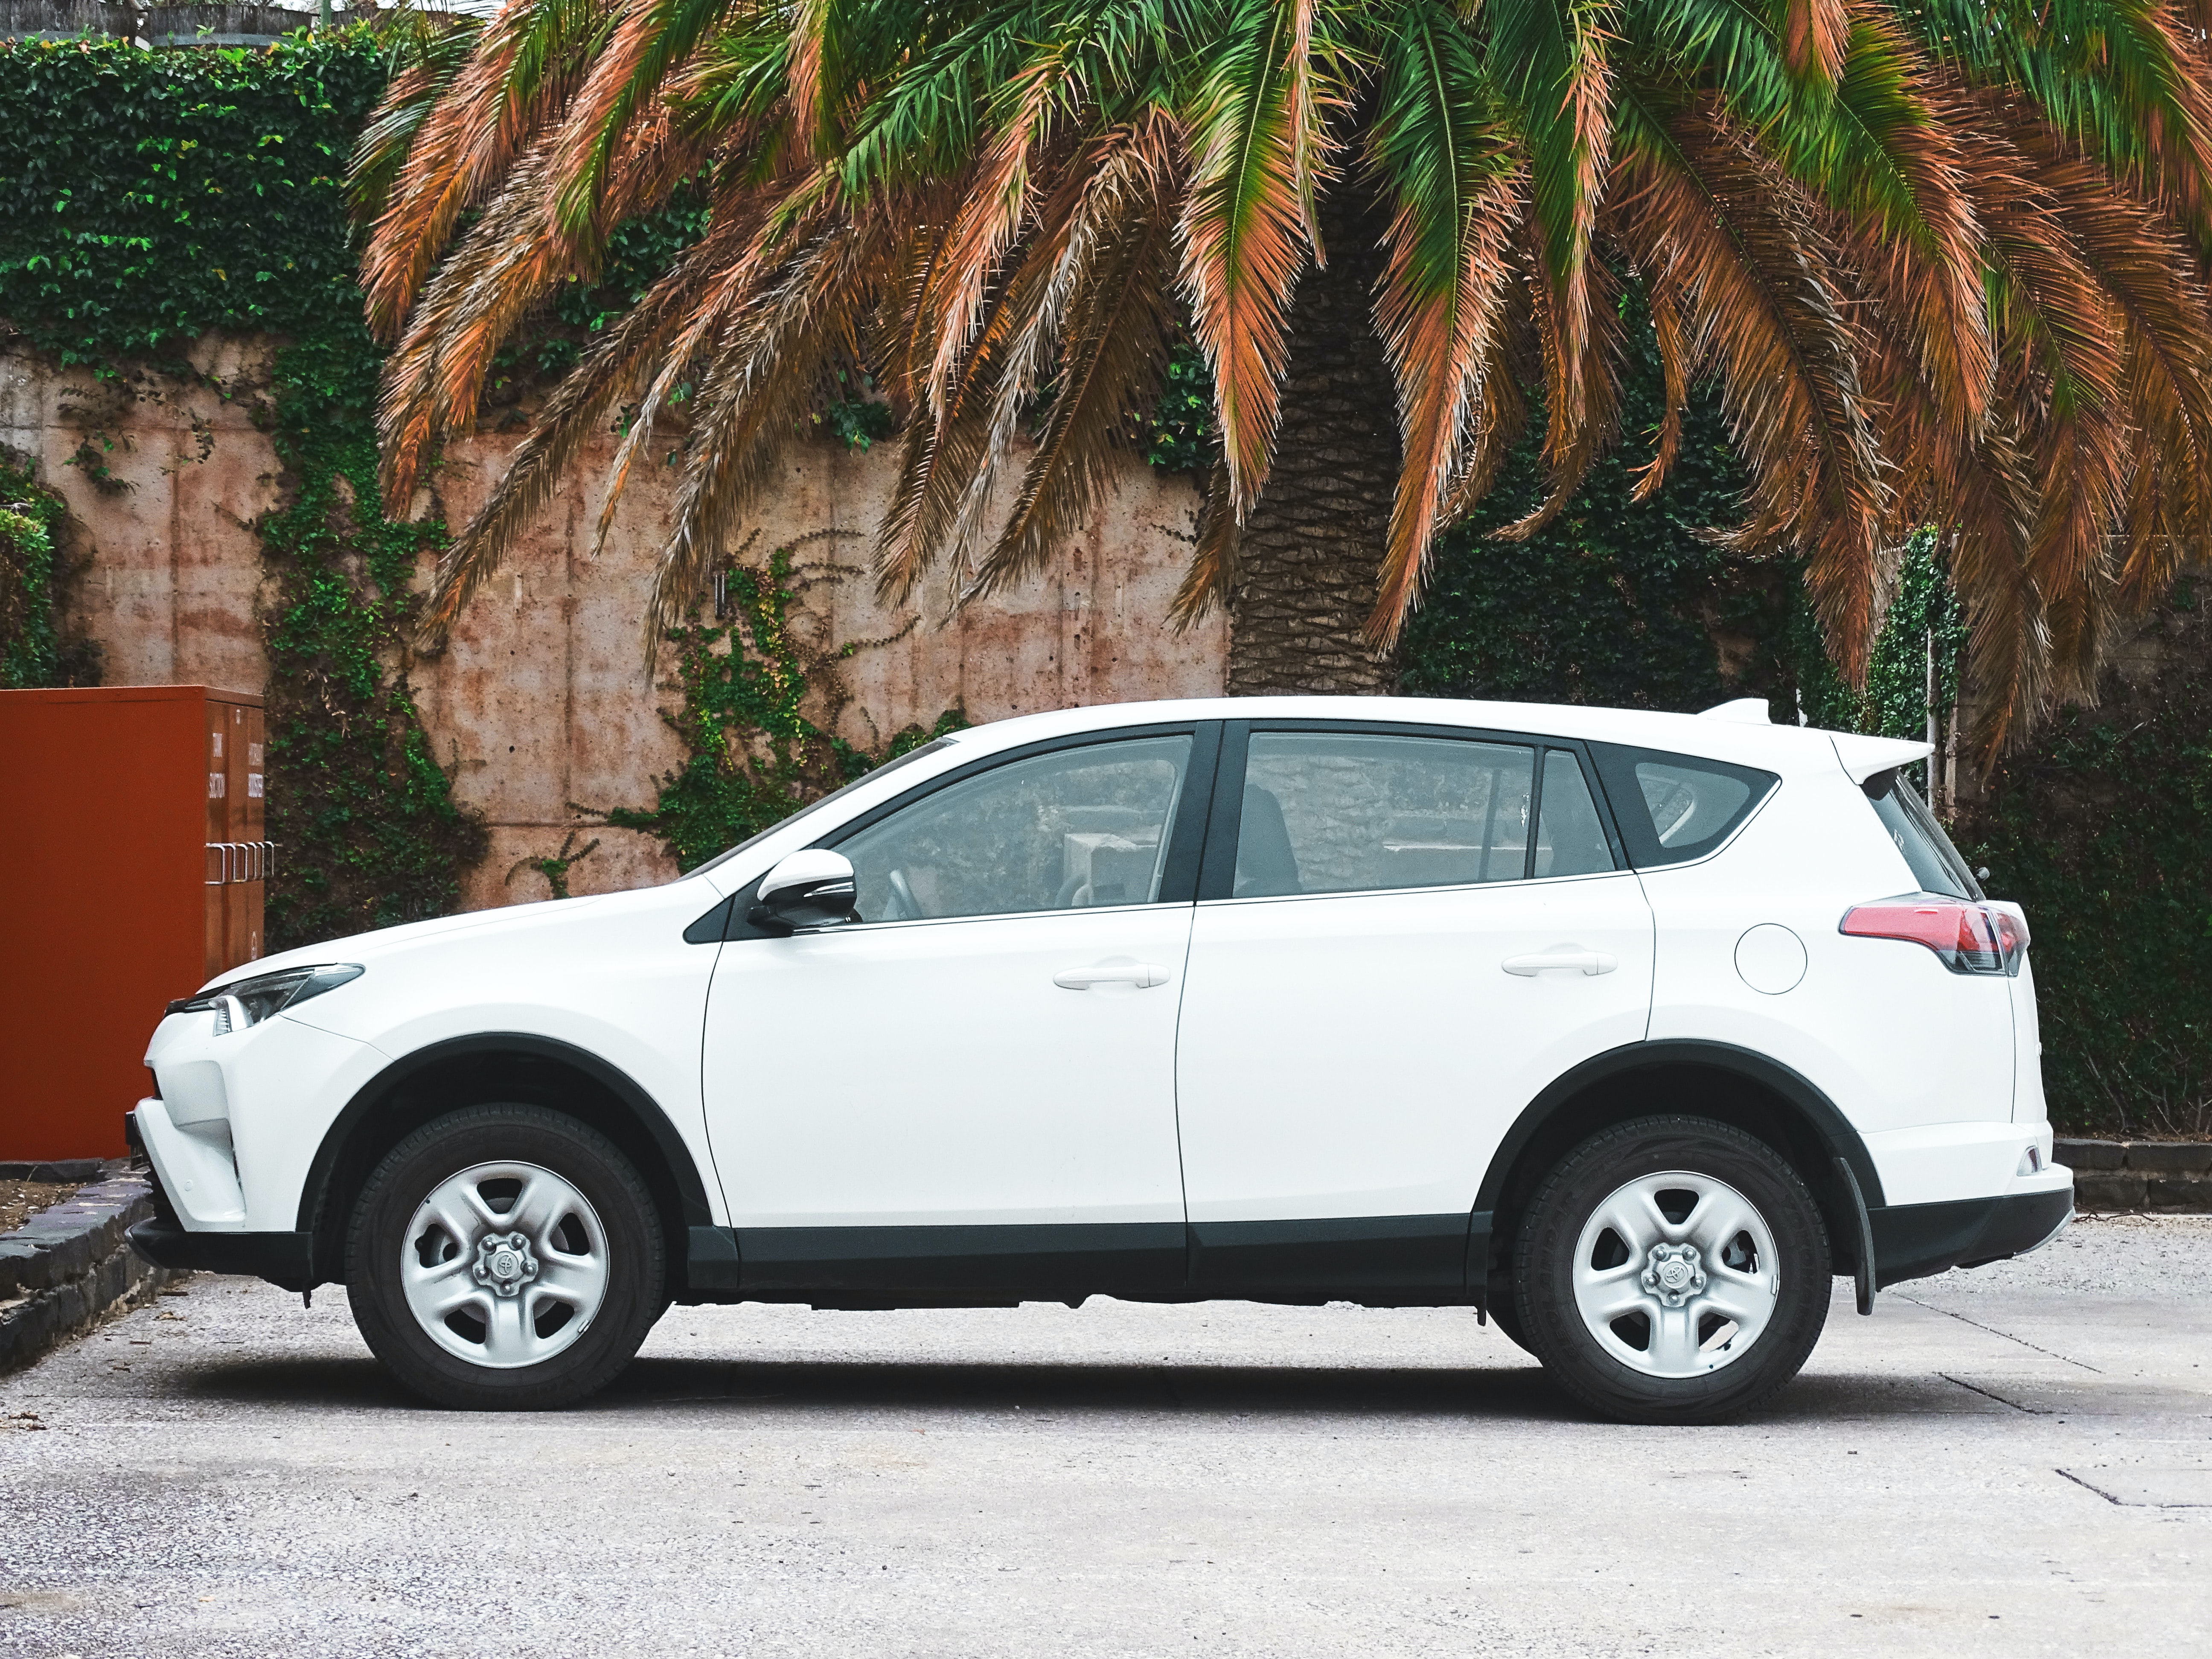
\includegraphics[width=0.7\columnwidth]{Image1}

%\VAR{testVar}


\begin{tabular}{| m{3cm} | m{3cm} |}
\hline

Title  &  Value   \\

\hline
Camera Make  & \VAR{make1}   \\
\hline
Camera Model  & \VAR{model1}   \\
\hline
Exposure time  & \VAR{exposure_time1}  \\
\hline
aperture & \VAR{aperture1} \\
\hline


\end{tabular}


\end{center}

\pagebreak

\begin{center}
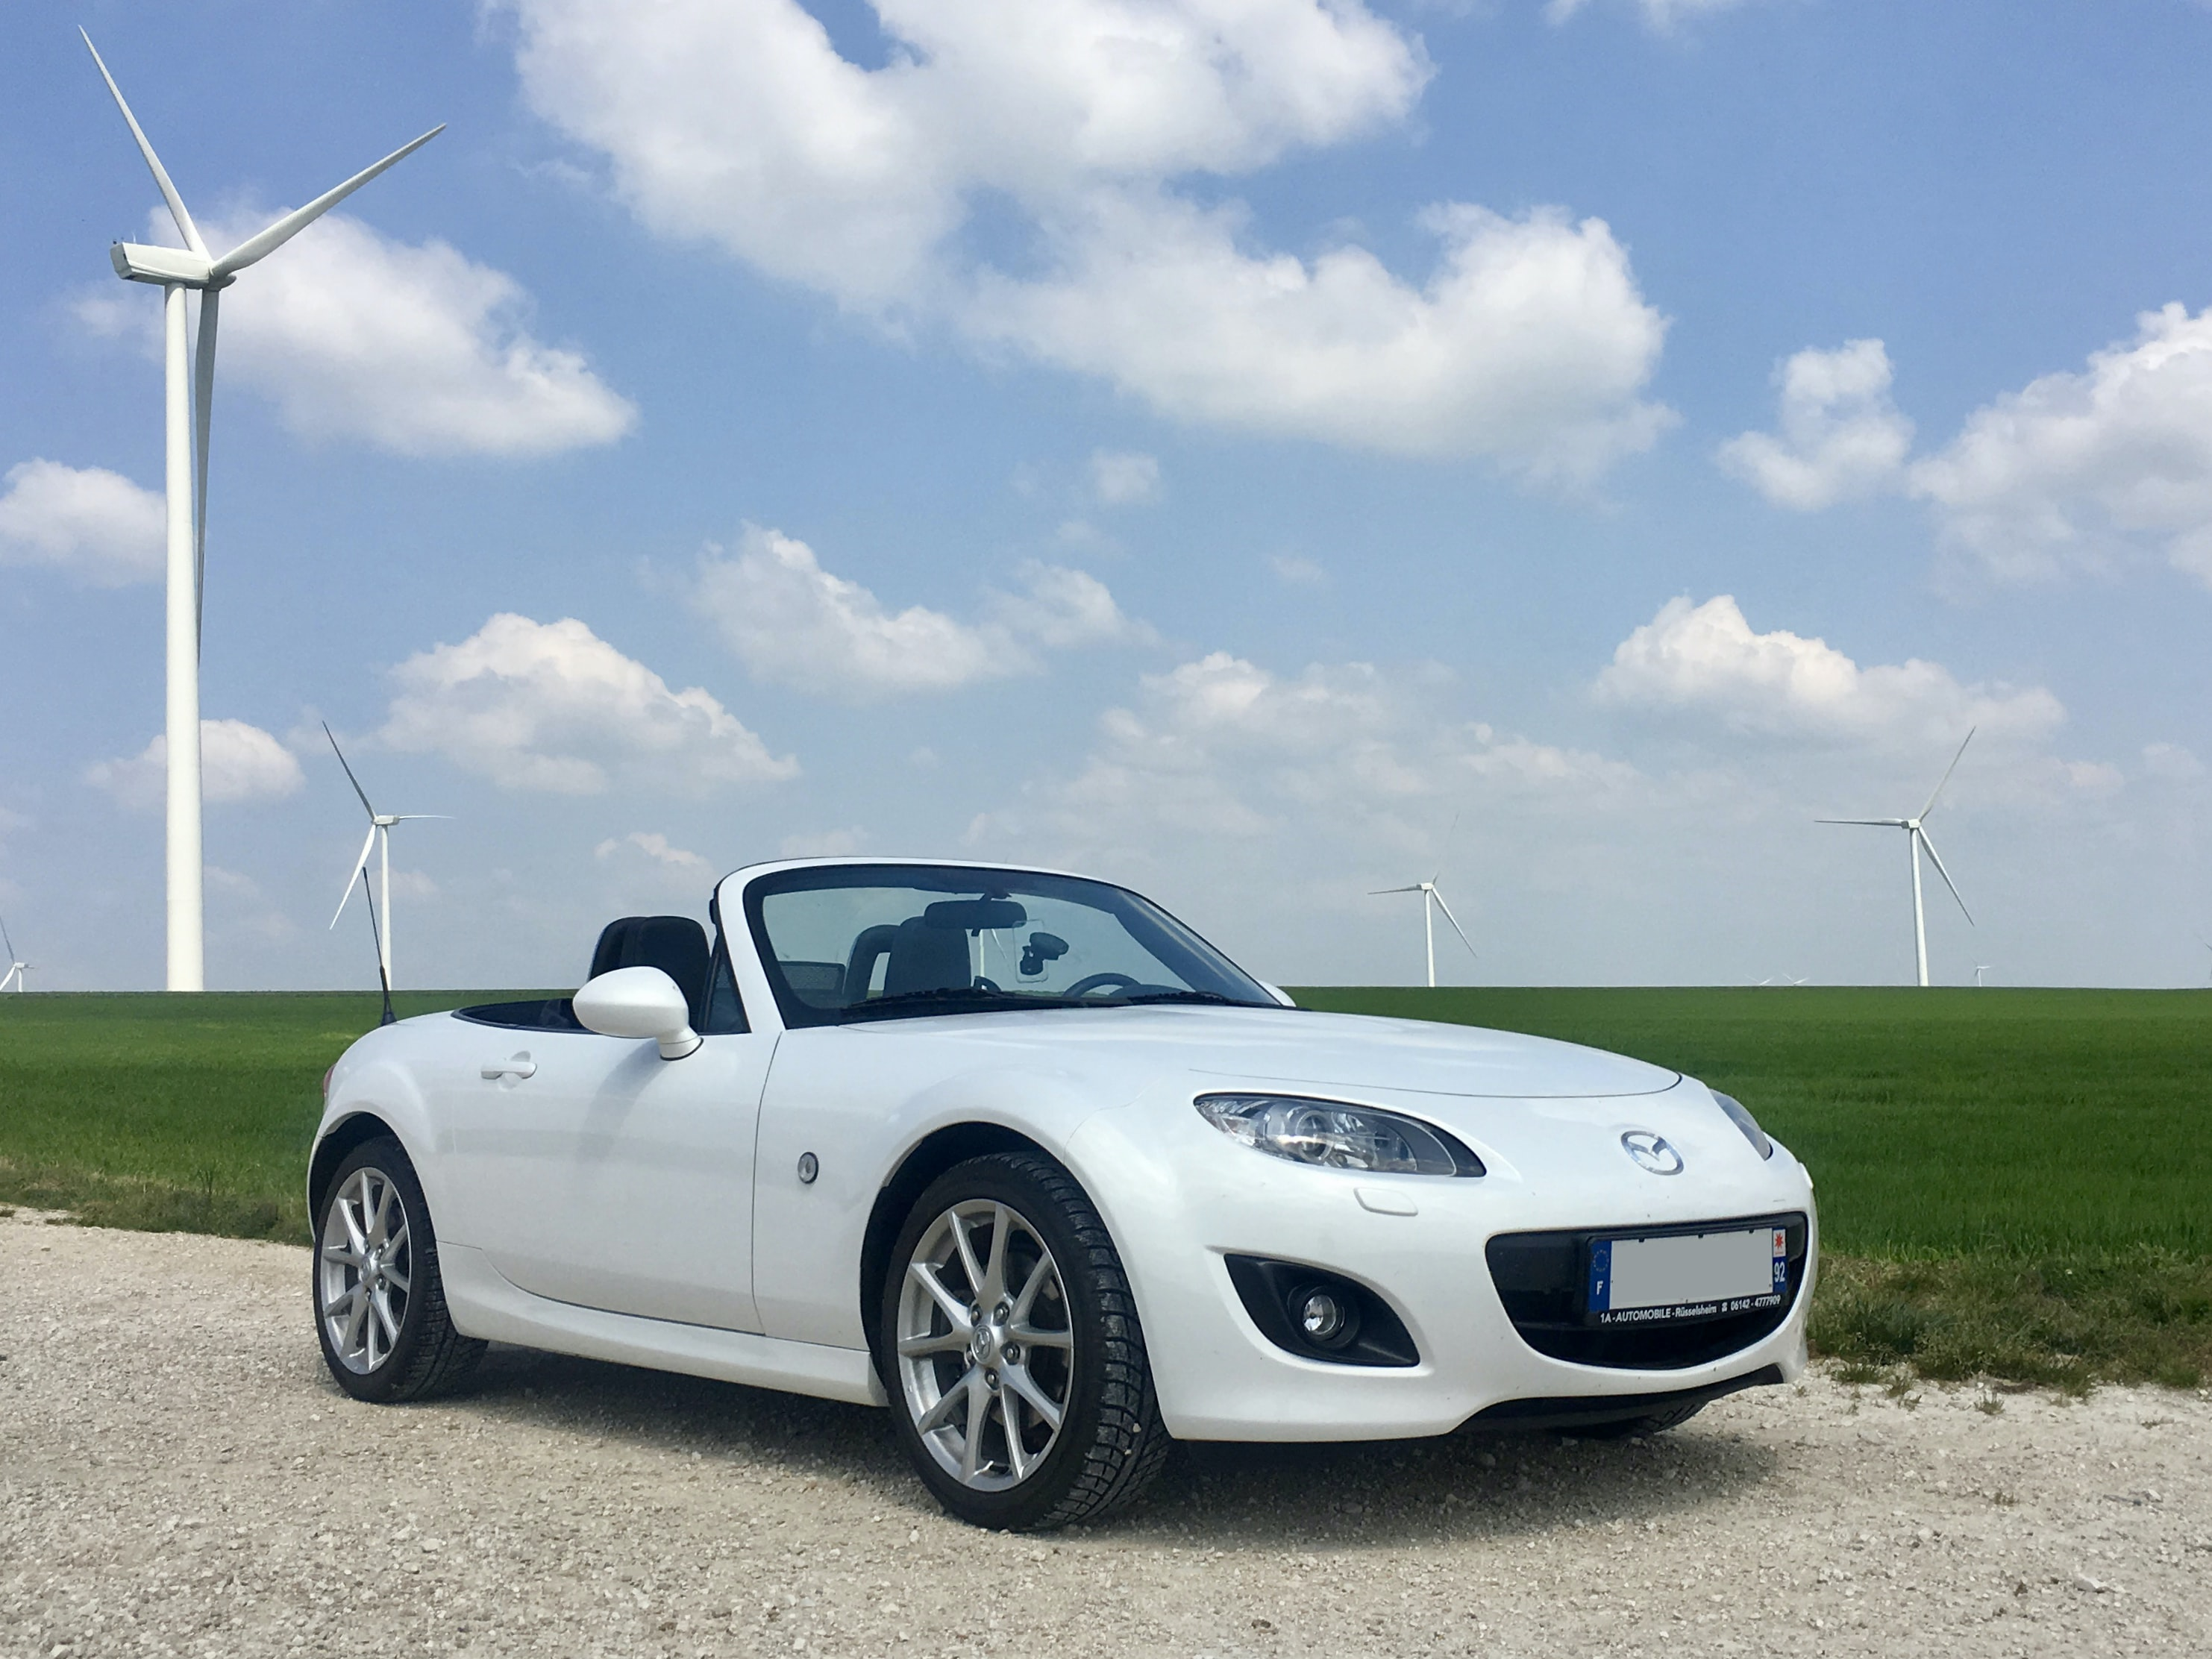
\includegraphics[width=0.7\columnwidth]{Image2}
\newline
\newline
\newline
\newline
\newline

\begin{tabular}{| m{3cm} | m{3cm} |}
\hline

Title  &  Value   \\

\hline
Camera Make  & \VAR{make2}   \\
\hline
Camera Model  & \VAR{model2}   \\
\hline
Exposure time  & \VAR{exposure_time2}  \\
\hline
aperture & \VAR{aperture2} \\
\hline

\end{tabular}


\end{center}

\newpage

\begin{center}
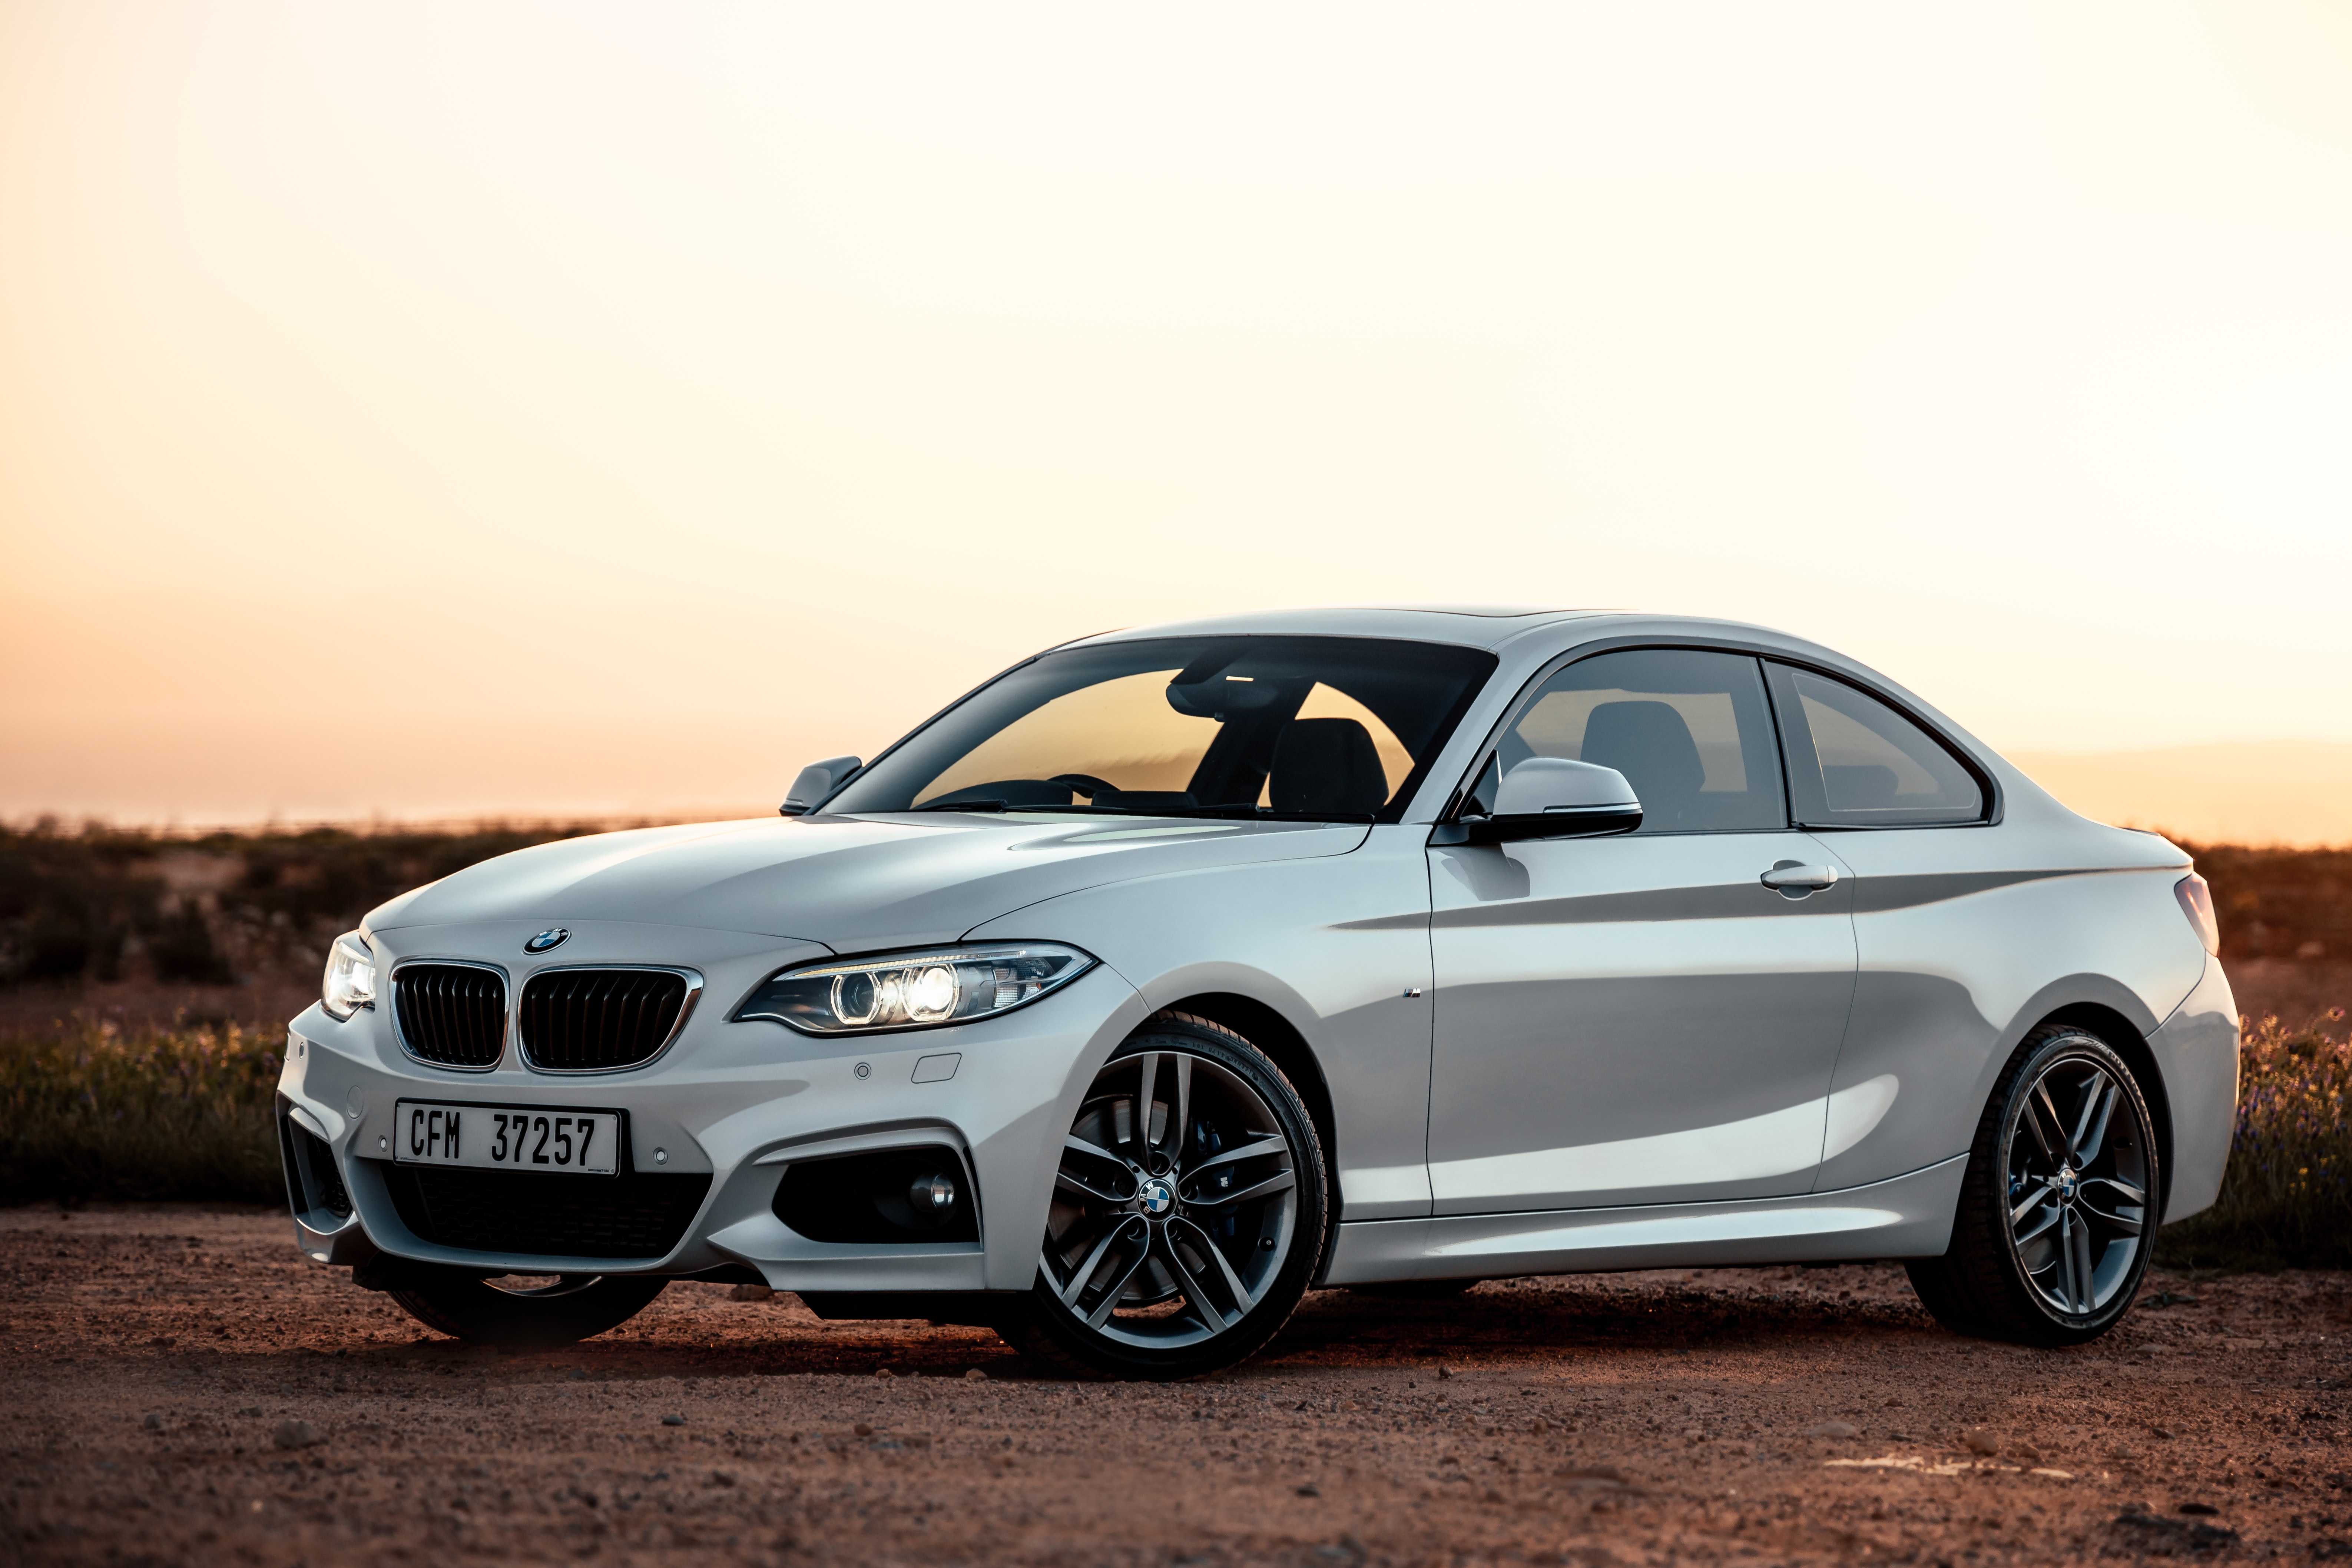
\includegraphics[width=0.7\columnwidth]{Image3}
\newline
\newline
\newline
\newline
\newline
\begin{tabular}{| m{3cm} | m{3cm} |}
\hline

Title  &  Value   \\

Title  &  Value   \\

\hline
Camera Make  & \VAR{make3}   \\
\hline
Camera Model  & \VAR{model3}   \\
\hline
Exposure time  & \VAR{exposure_time3}  \\
\hline
aperture & \VAR{aperture3} \\
\hline


\end{tabular}


\end{center}

\pagebreak

\begin{center}
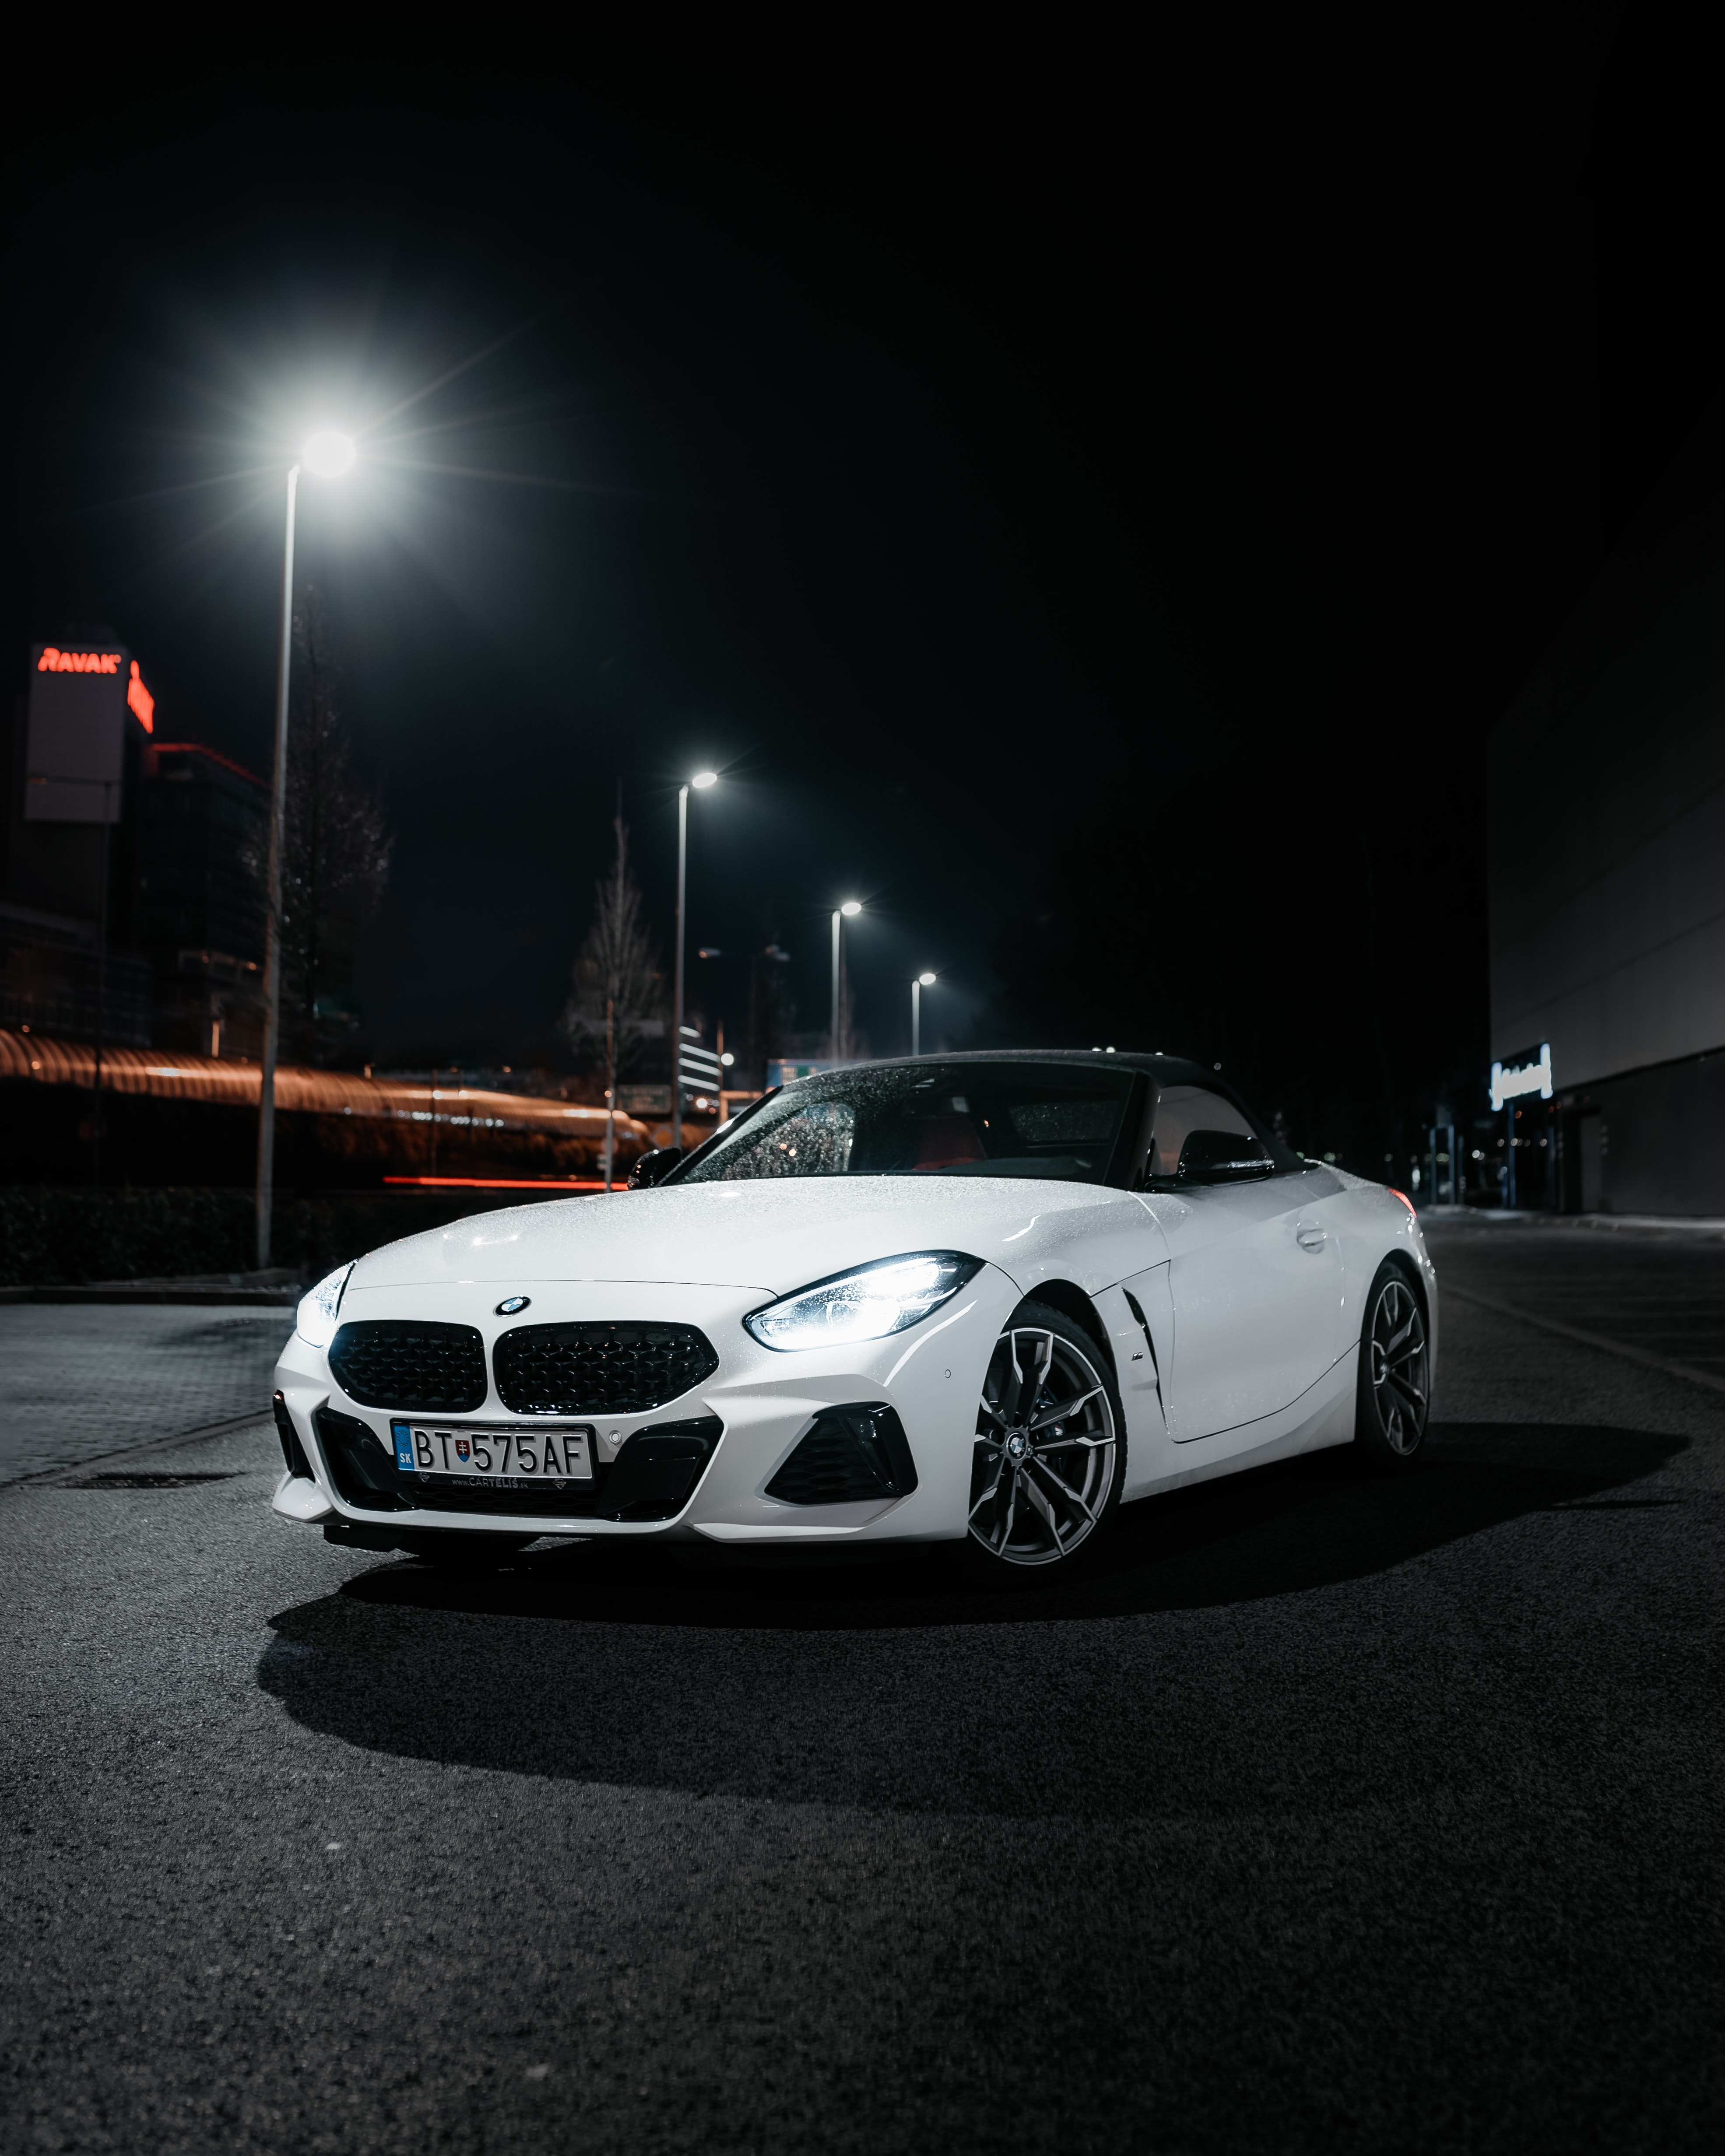
\includegraphics[width=0.7\columnwidth]{Image4}
\newline
\newline
\newline
\newline
\newline

\begin{tabular}{| m{3cm} | m{3cm} |}
\hline

Title  &  Value   \\

\hline
Camera Make  & \VAR{make4}   \\
\hline
Camera Model  & \VAR{model4}   \\
\hline
Exposure time  & \VAR{exposure_time4}  \\
\hline
aperture & \VAR{aperture4} \\
\hline

\end{tabular}


\end{center}

\newpage

\begin{center}
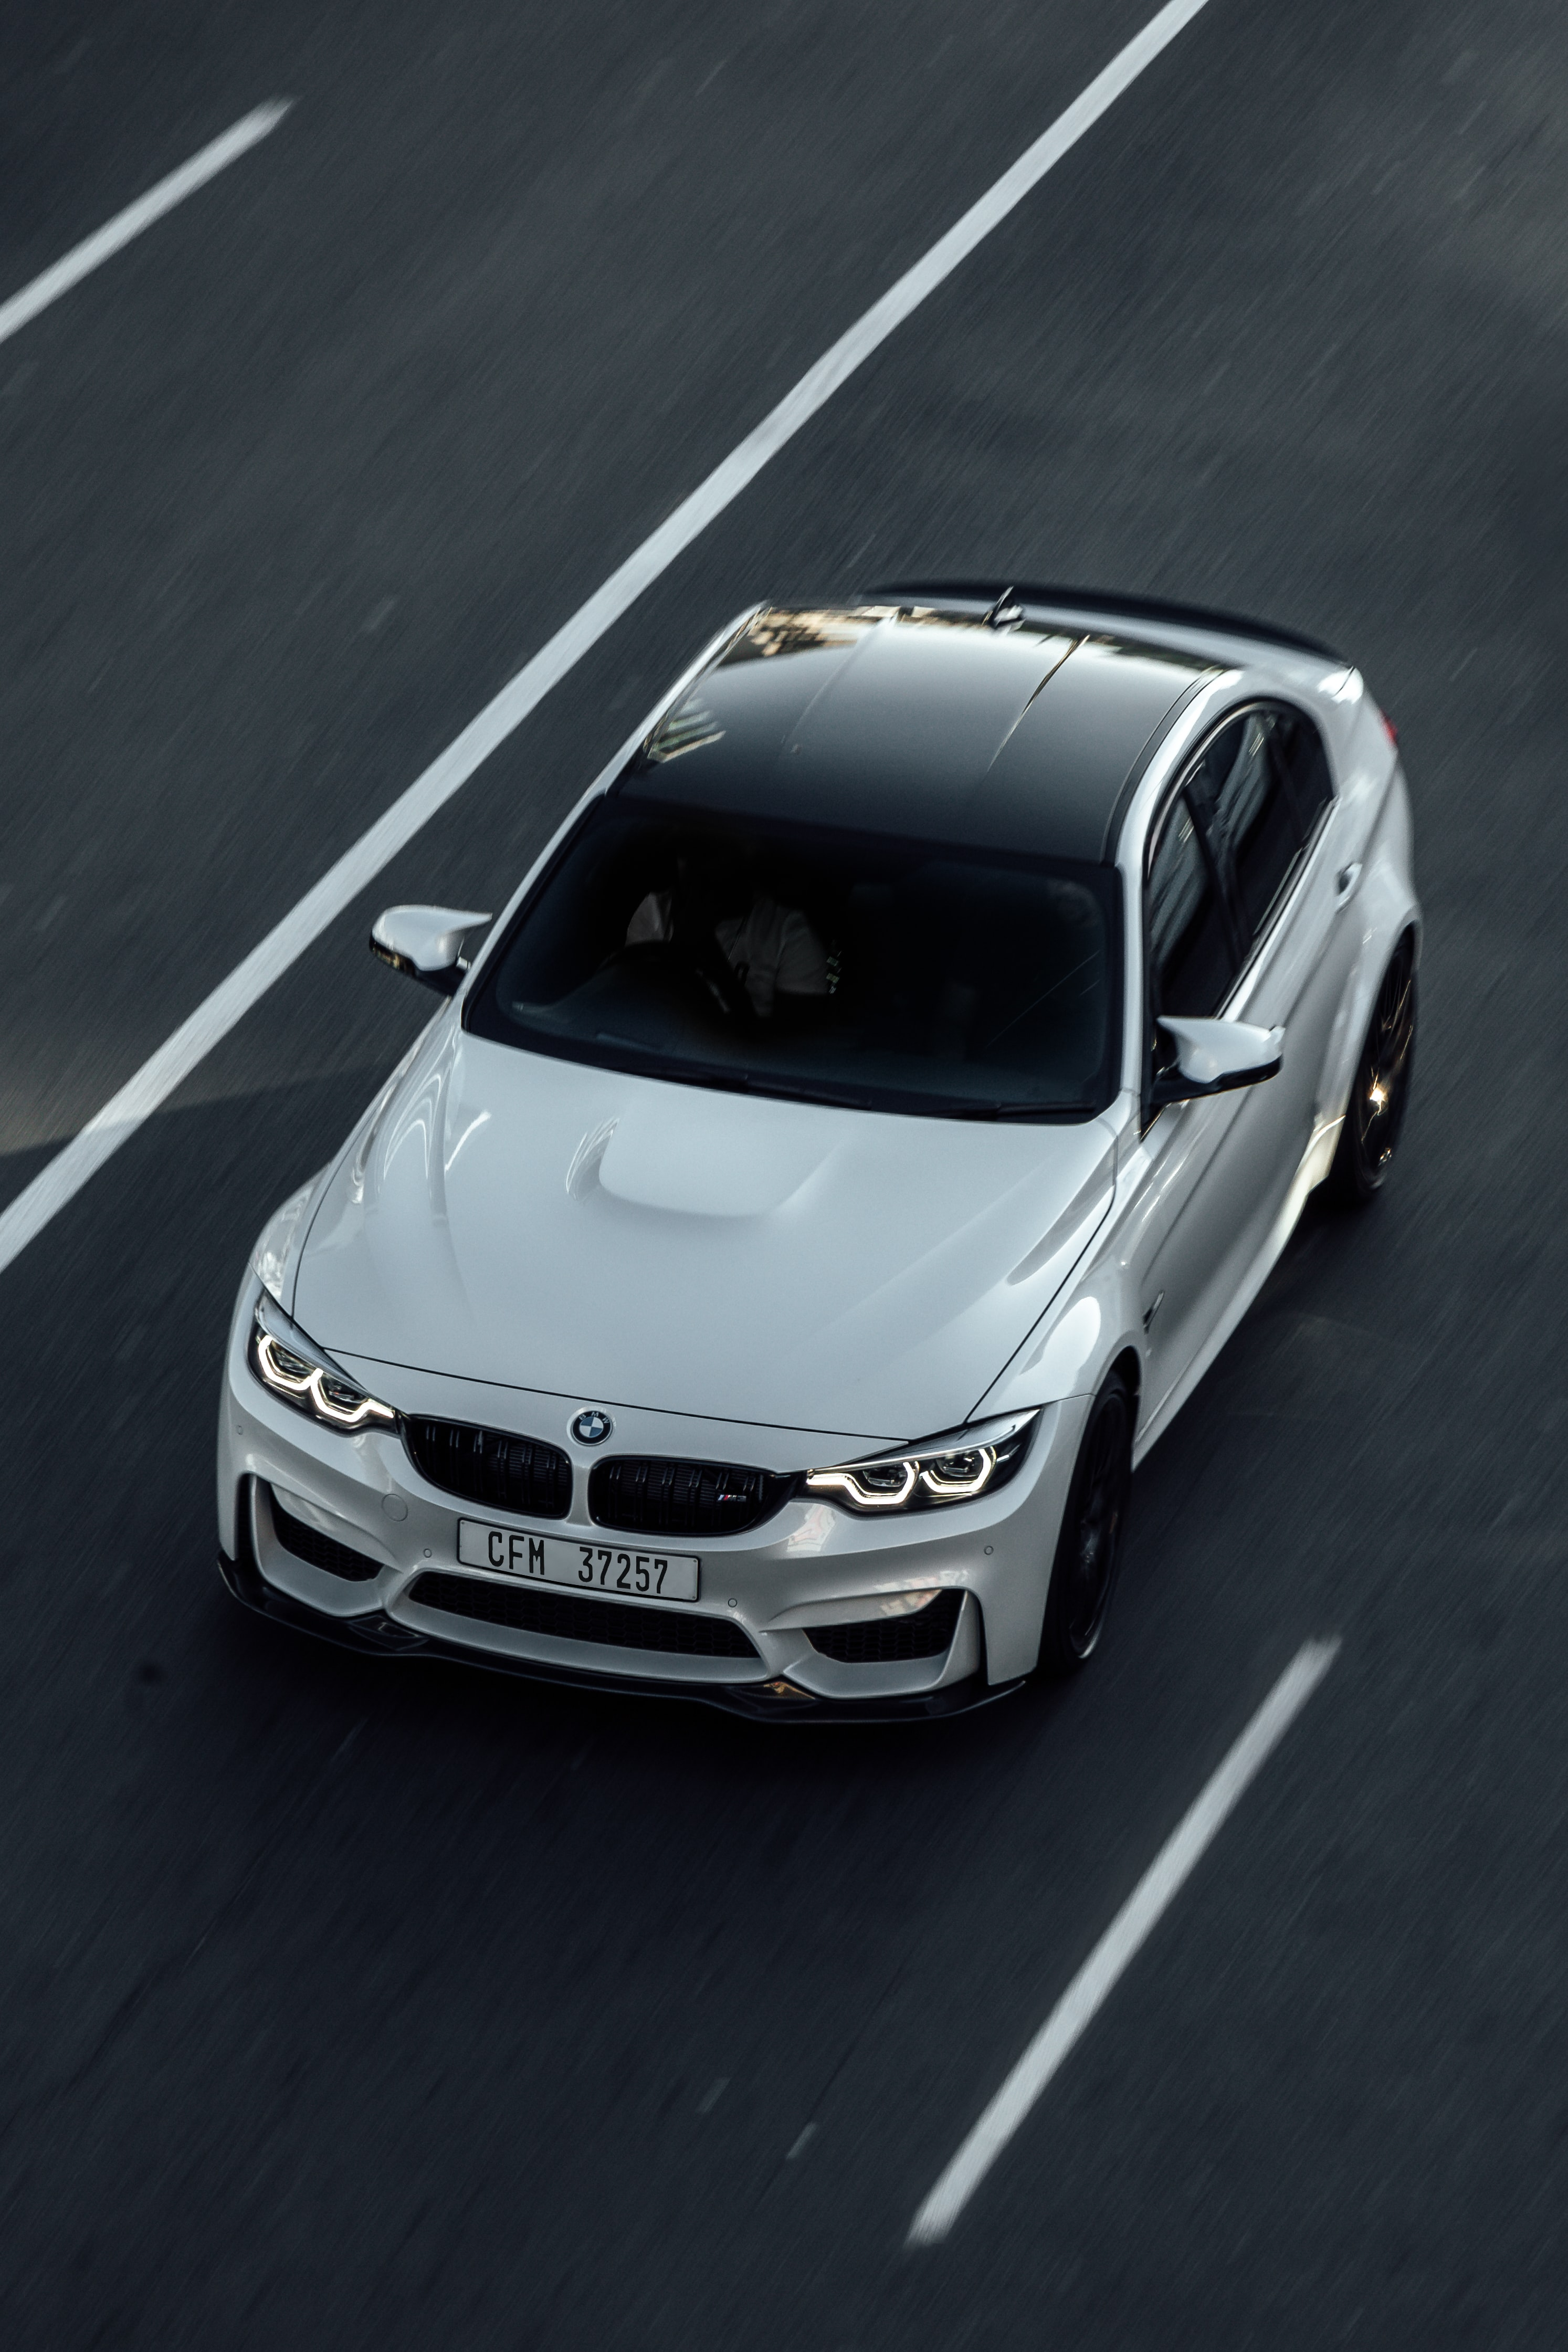
\includegraphics[width=0.7\columnwidth]{Image5}
\newline
\newline
\newline
\newline
\newline
\begin{tabular}{| m{3cm} | m{3cm} |}
\hline

Title  &  Value   \\

\hline
Camera Make  & \VAR{make5}   \\
\hline
Camera Model  & \VAR{model5}   \\
\hline
Exposure time  & \VAR{exposure_time5}  \\
\hline
aperture & \VAR{aperture5} \\
\hline


\end{tabular}


\end{center}

\pagebreak

\begin{center}
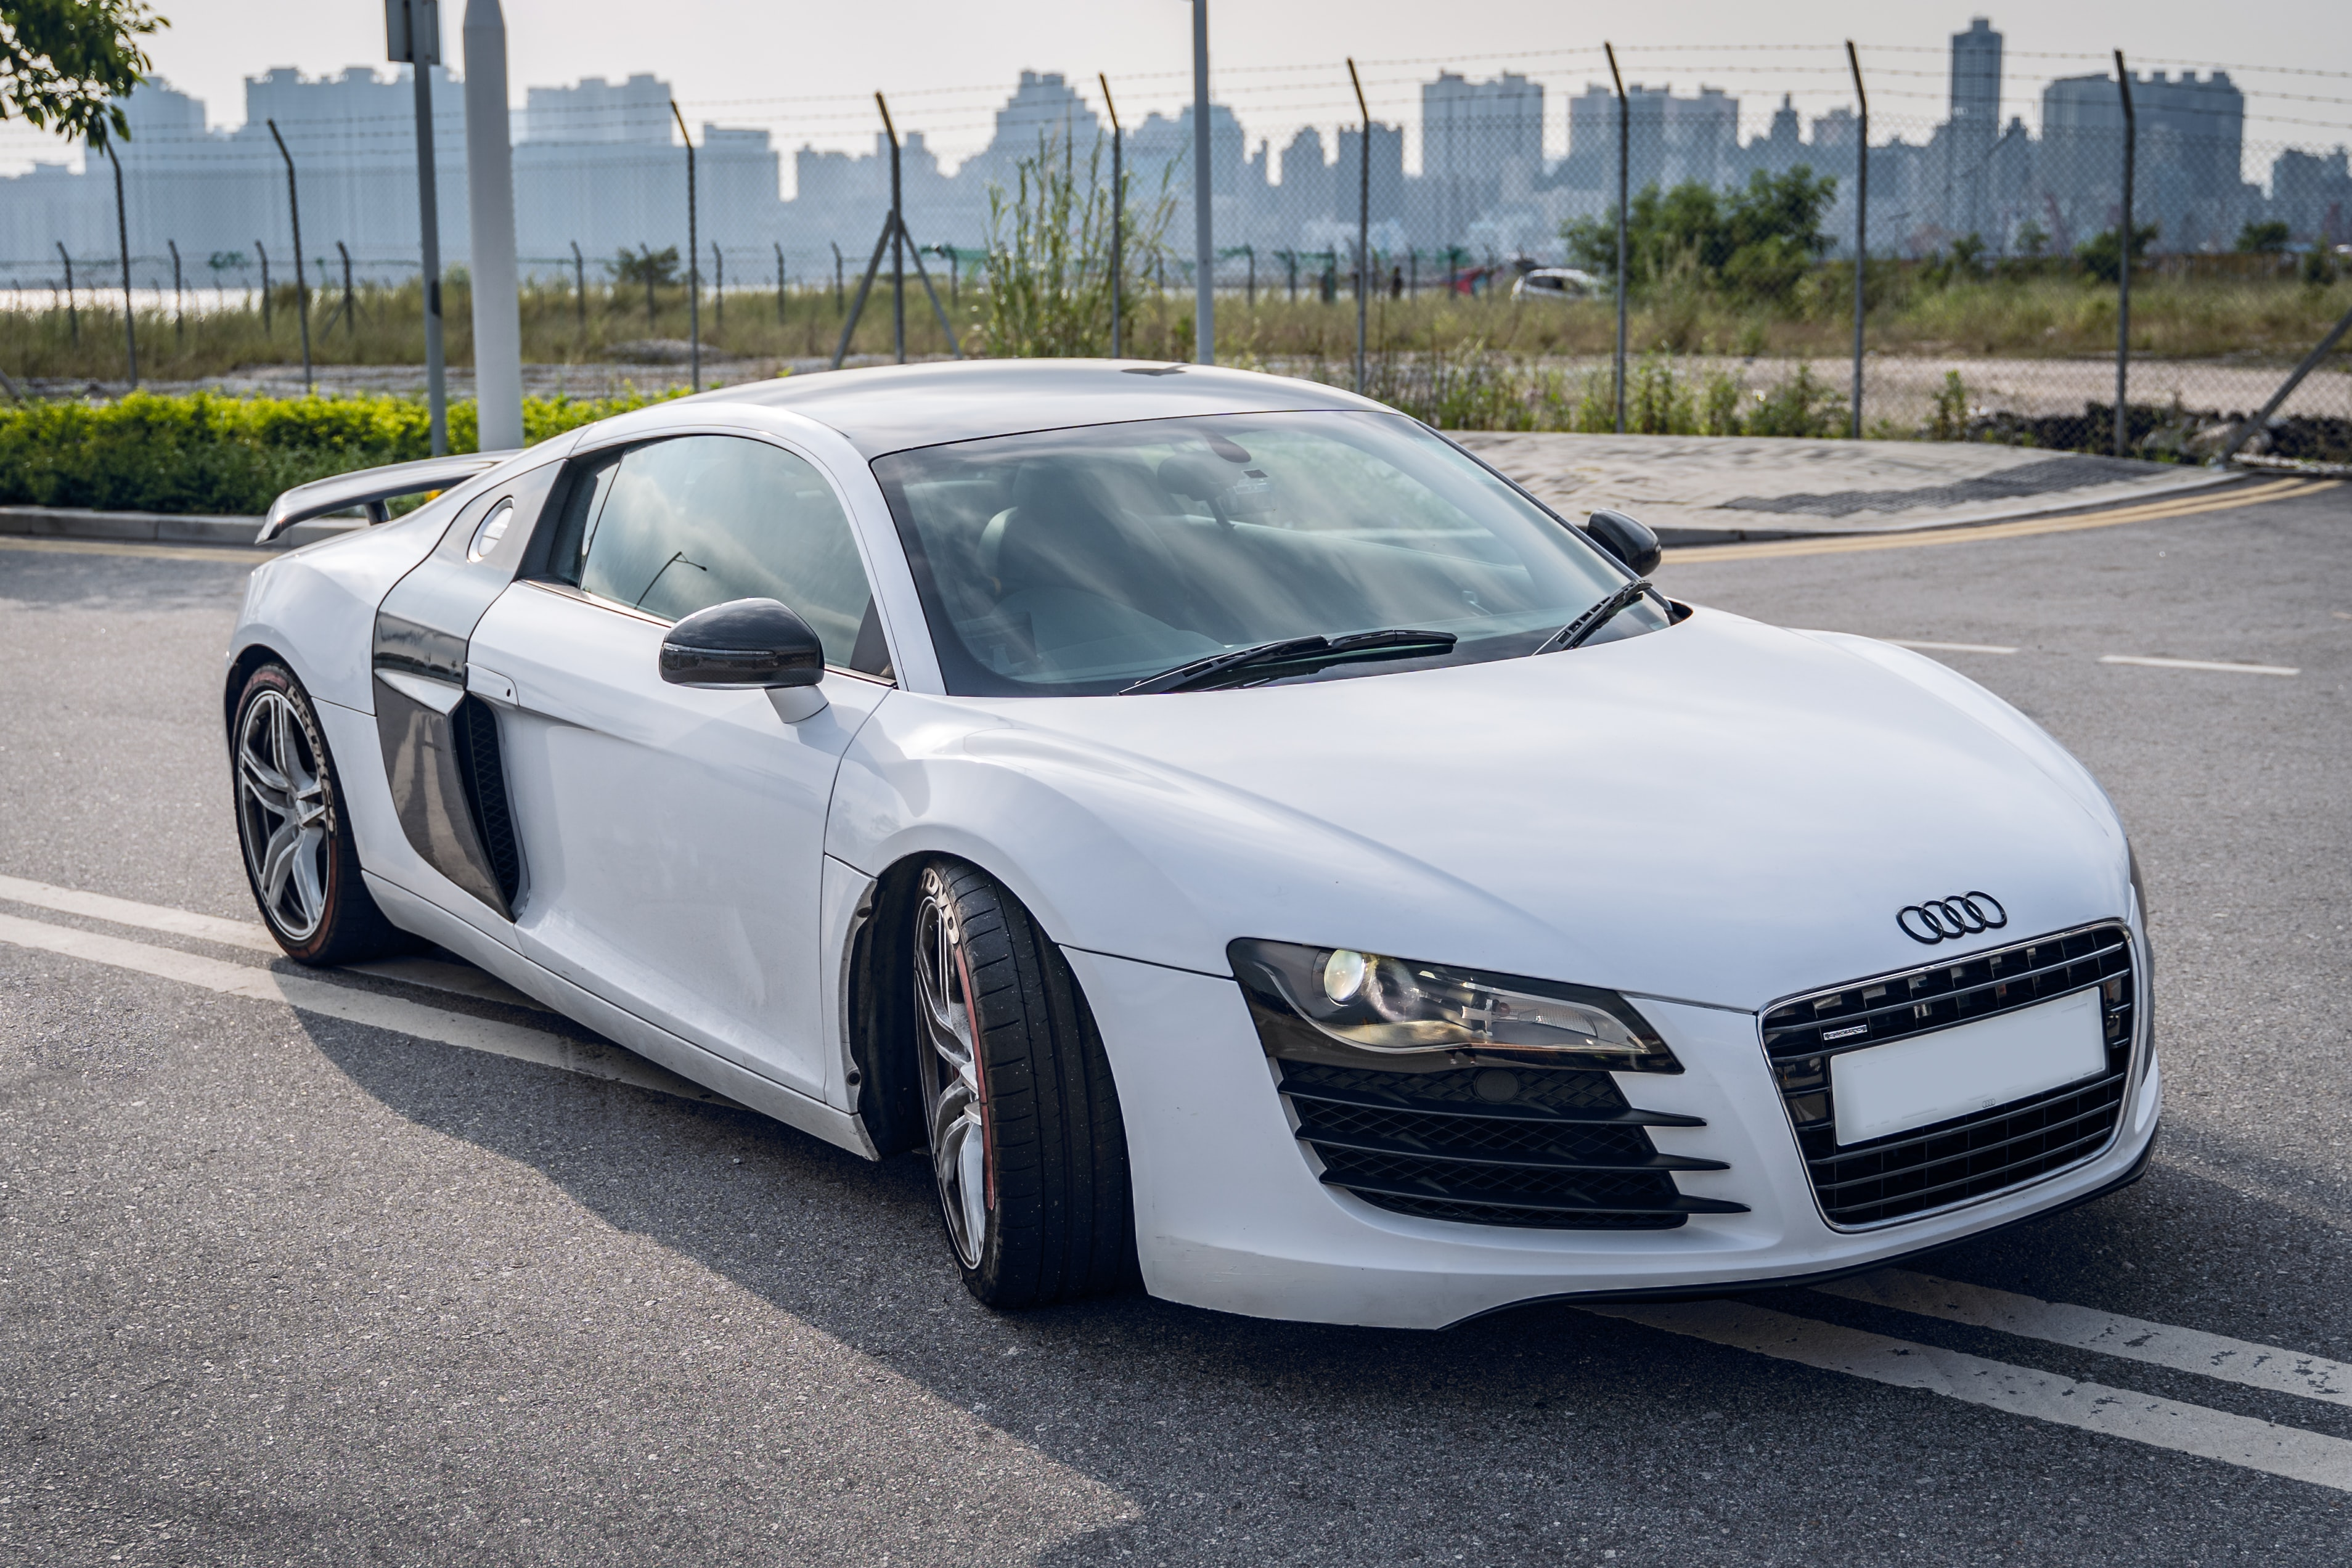
\includegraphics[width=0.7\columnwidth]{Image6}
\newline
\newline
\newline
\newline
\newline

\begin{tabular}{| m{3cm} | m{3cm} |}
\hline

Title  &  Value   \\

\hline
Camera Make  & \VAR{make6}   \\
\hline
Camera Model  & \VAR{model6}   \\
\hline
Exposure time  & \VAR{exposure_time6}  \\
\hline
aperture & \VAR{aperture6} \\
\hline

\end{tabular}


\end{center}

\newpage

\begin{center}
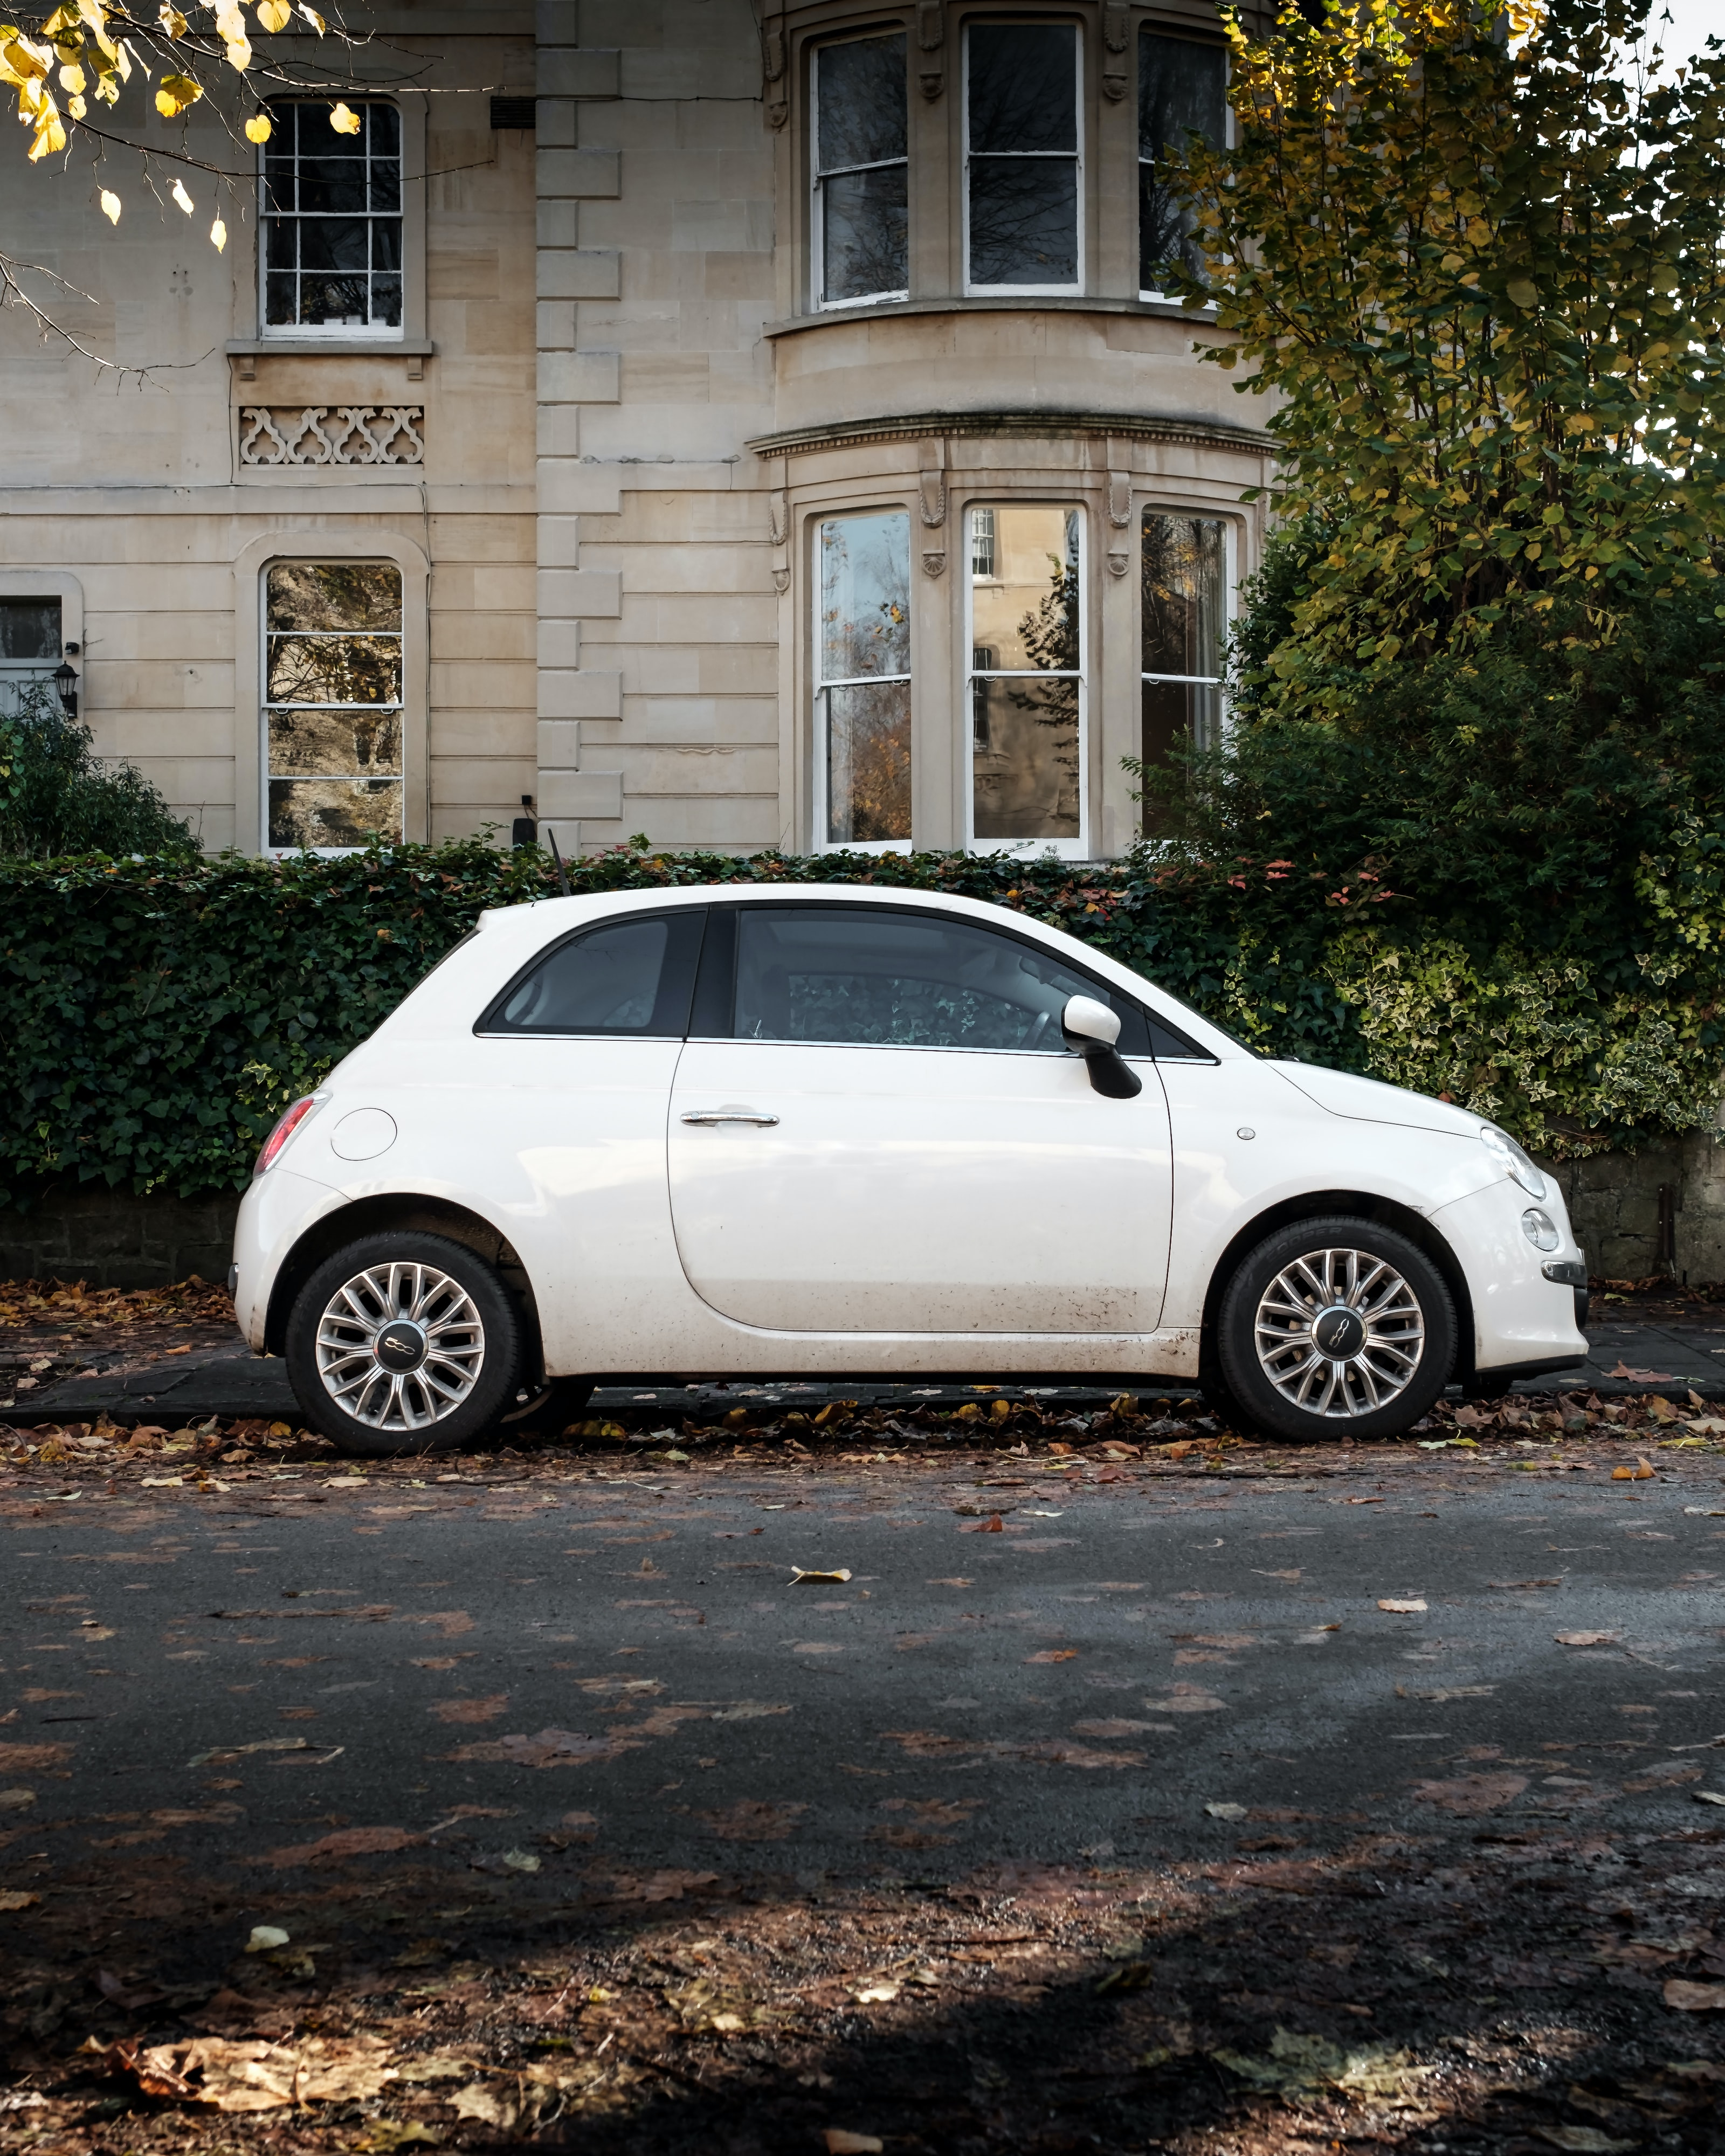
\includegraphics[width=0.7\columnwidth]{Image7}
\newline
\newline
\newline
\newline
\newline
\begin{tabular}{| m{3cm} | m{3cm} |}
\hline

Title  &  Value   \\

\hline
Camera Make  & \VAR{make7}   \\
\hline
Camera Model  & \VAR{model7}   \\
\hline
Exposure time  & \VAR{exposure_time7}  \\
\hline
aperture & \VAR{aperture7} \\
\hline


\end{tabular}


\end{center}

\pagebreak

\begin{center}
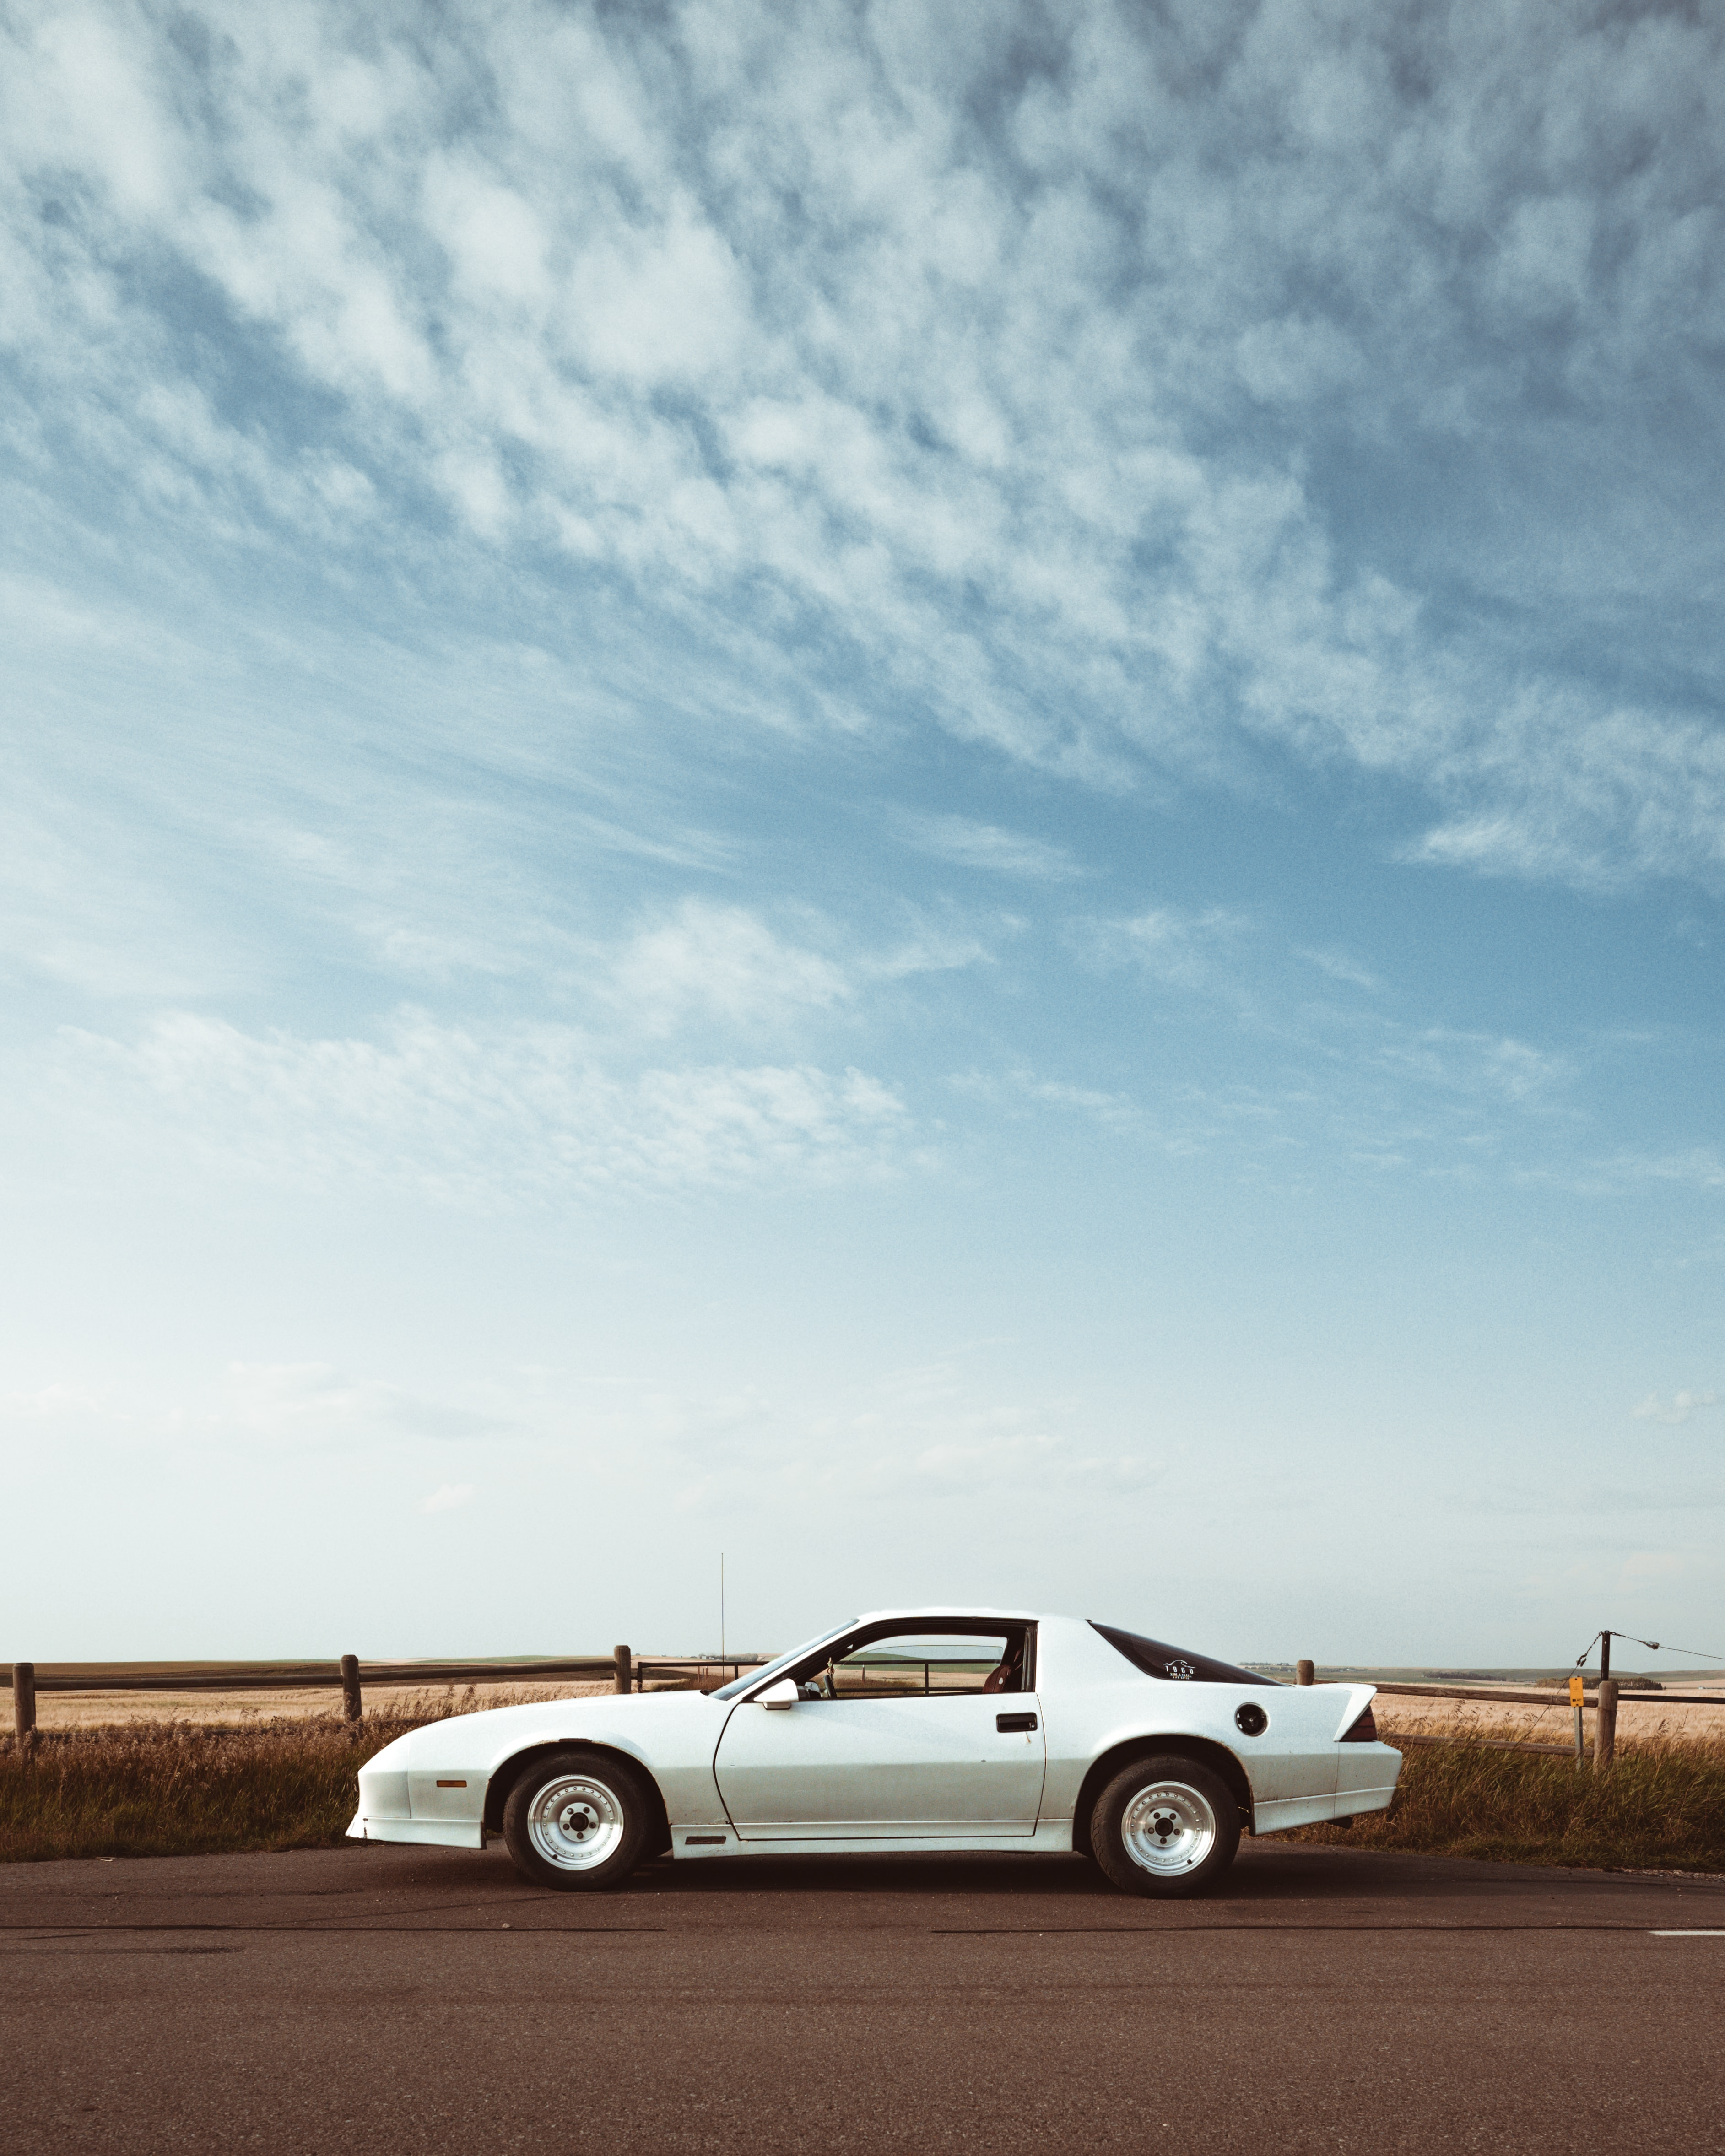
\includegraphics[width=0.7\columnwidth]{Image8}
\newline
\newline
\newline
\newline
\newline

\begin{tabular}{| m{3cm} | m{3cm} |}
\hline

Title  &  Value   \\

\hline
Camera Make  & \VAR{make8}   \\
\hline
Camera Model  & \VAR{model8}   \\
\hline
Exposure time  & \VAR{exposure_time8}  \\
\hline
aperture & \VAR{aperture8} \\
\hline

\end{tabular}


\end{center}

\newpage

\begin{center}
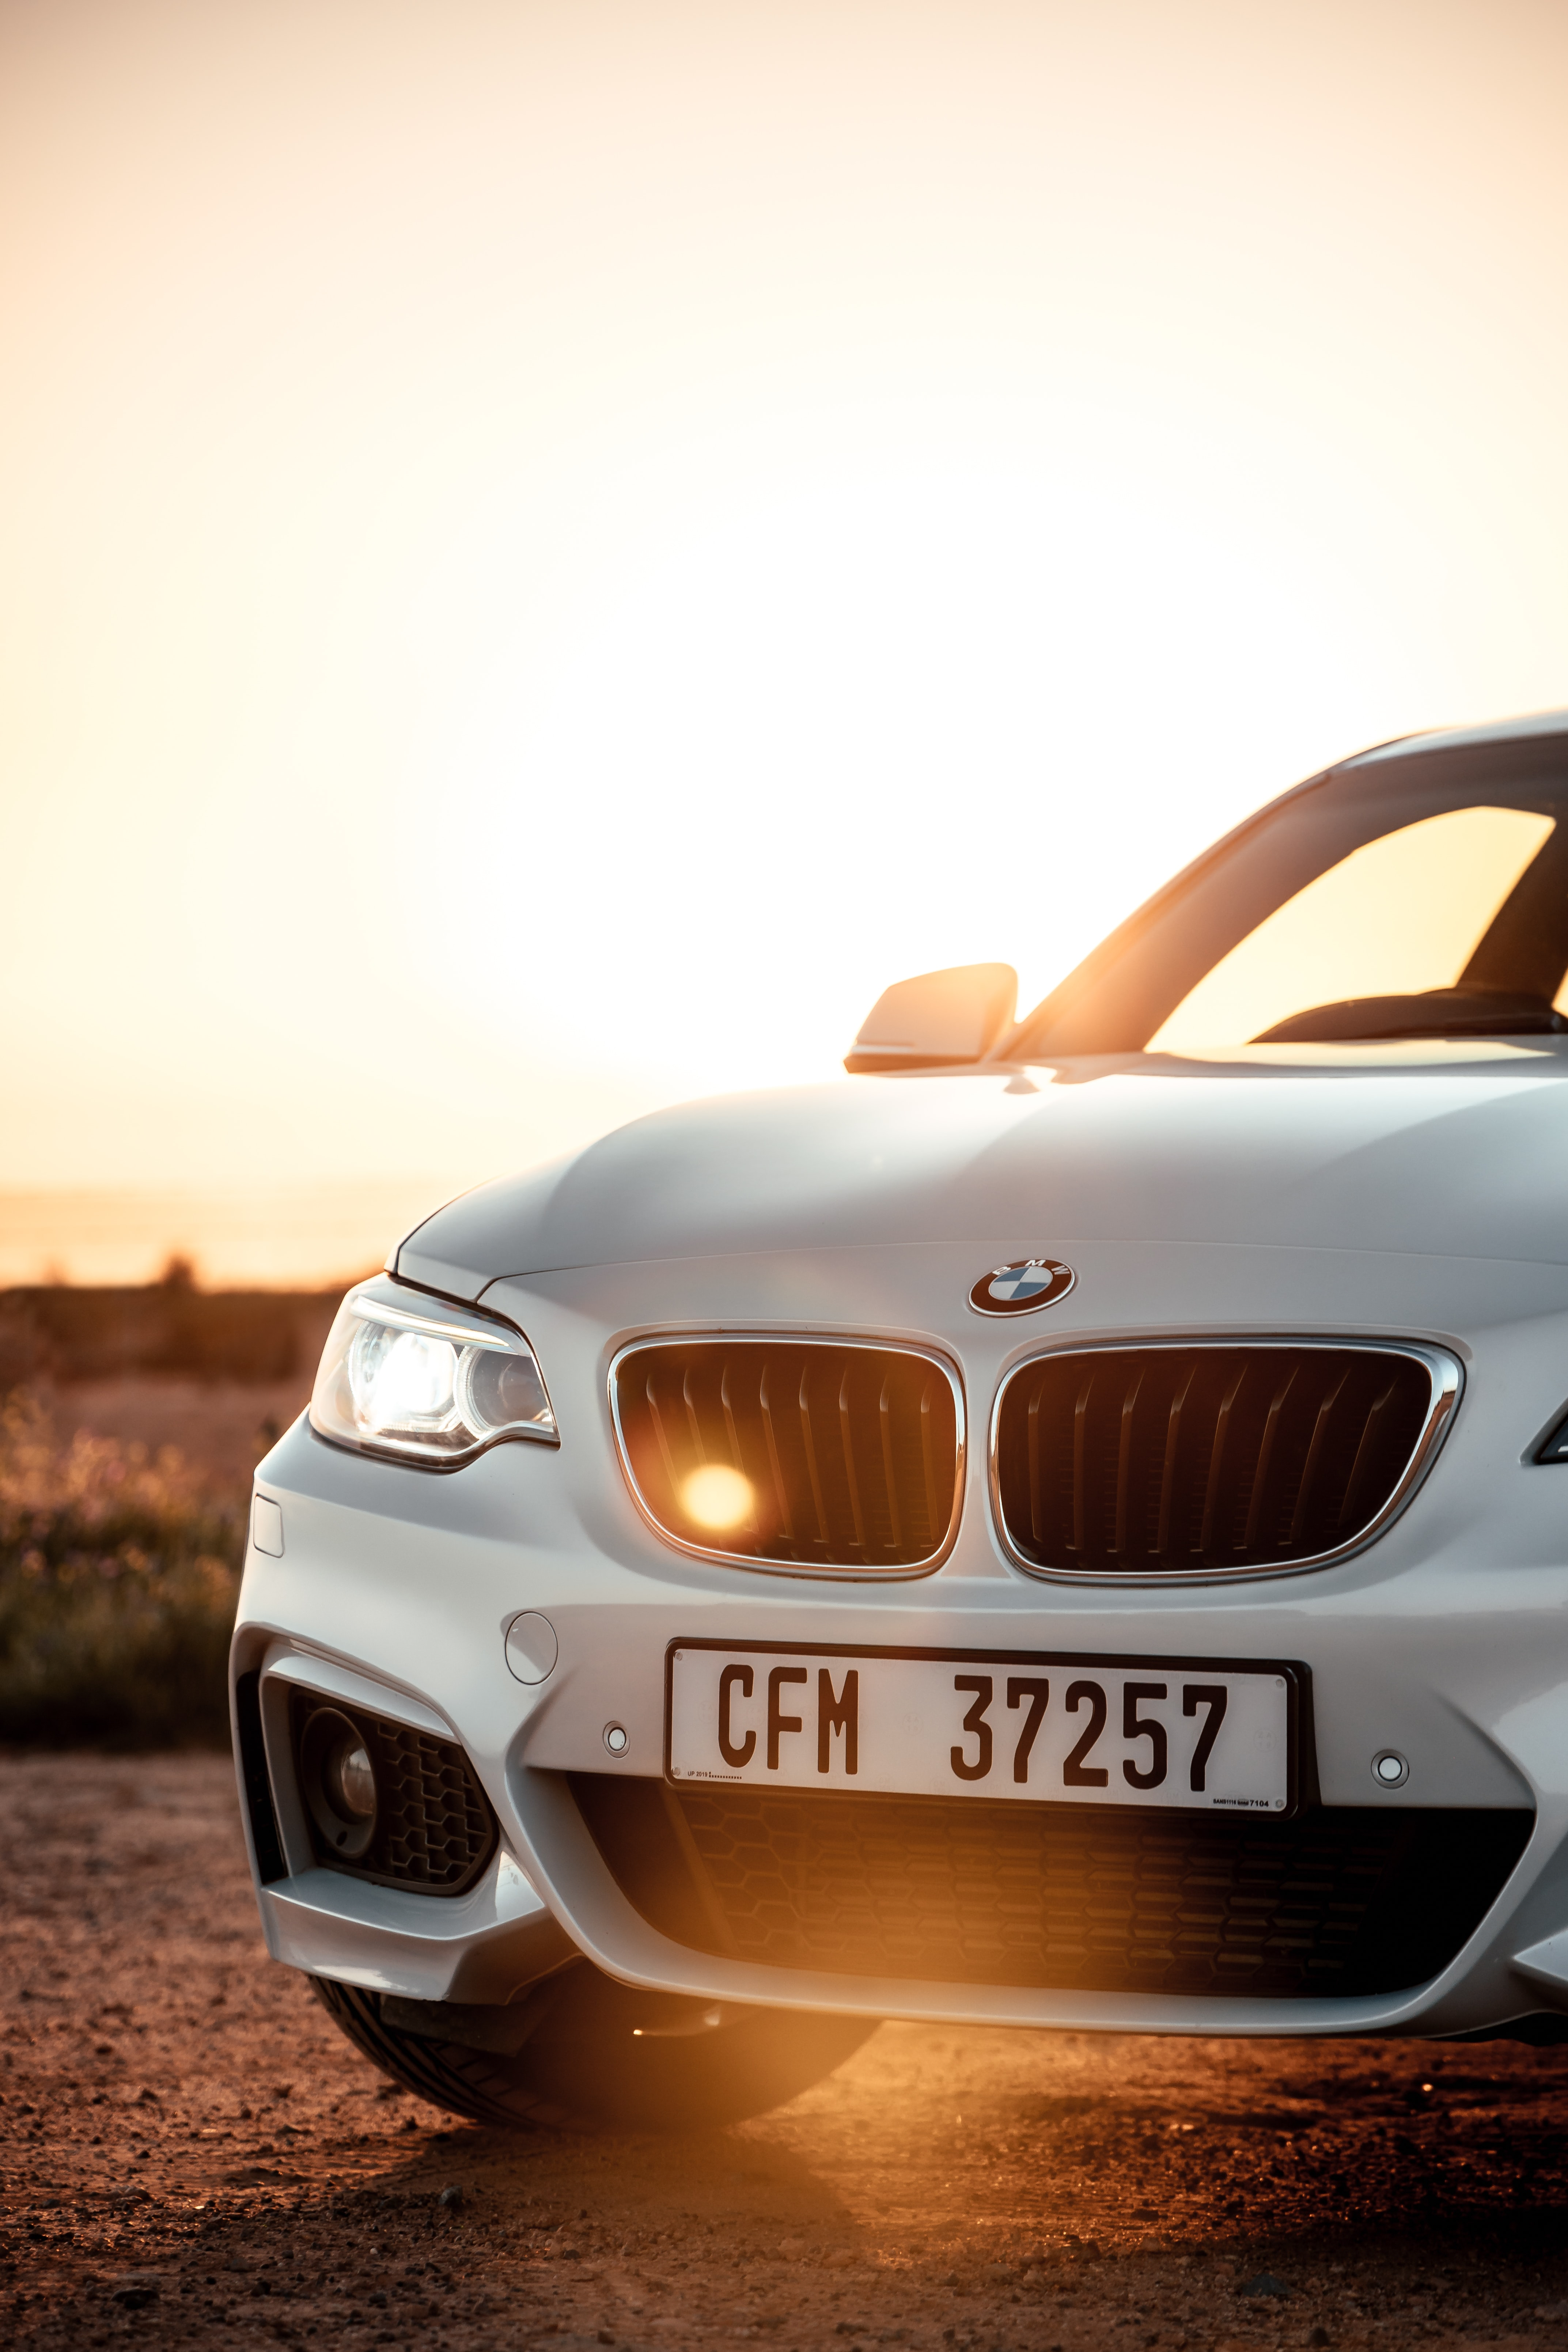
\includegraphics[width=0.7\columnwidth]{Image9}
\newline
\newline
\newline
\newline
\newline
\begin{tabular}{| m{3cm} | m{3cm} |}
\hline

Title  &  Value   \\

\hline
Camera Make  & \VAR{make9}   \\
\hline
Camera Model  & \VAR{model9}   \\
\hline
Exposure time  & \VAR{exposure_time9}  \\
\hline
aperture & \VAR{aperture9} \\
\hline


\end{tabular}


\end{center}

\pagebreak

\begin{center}
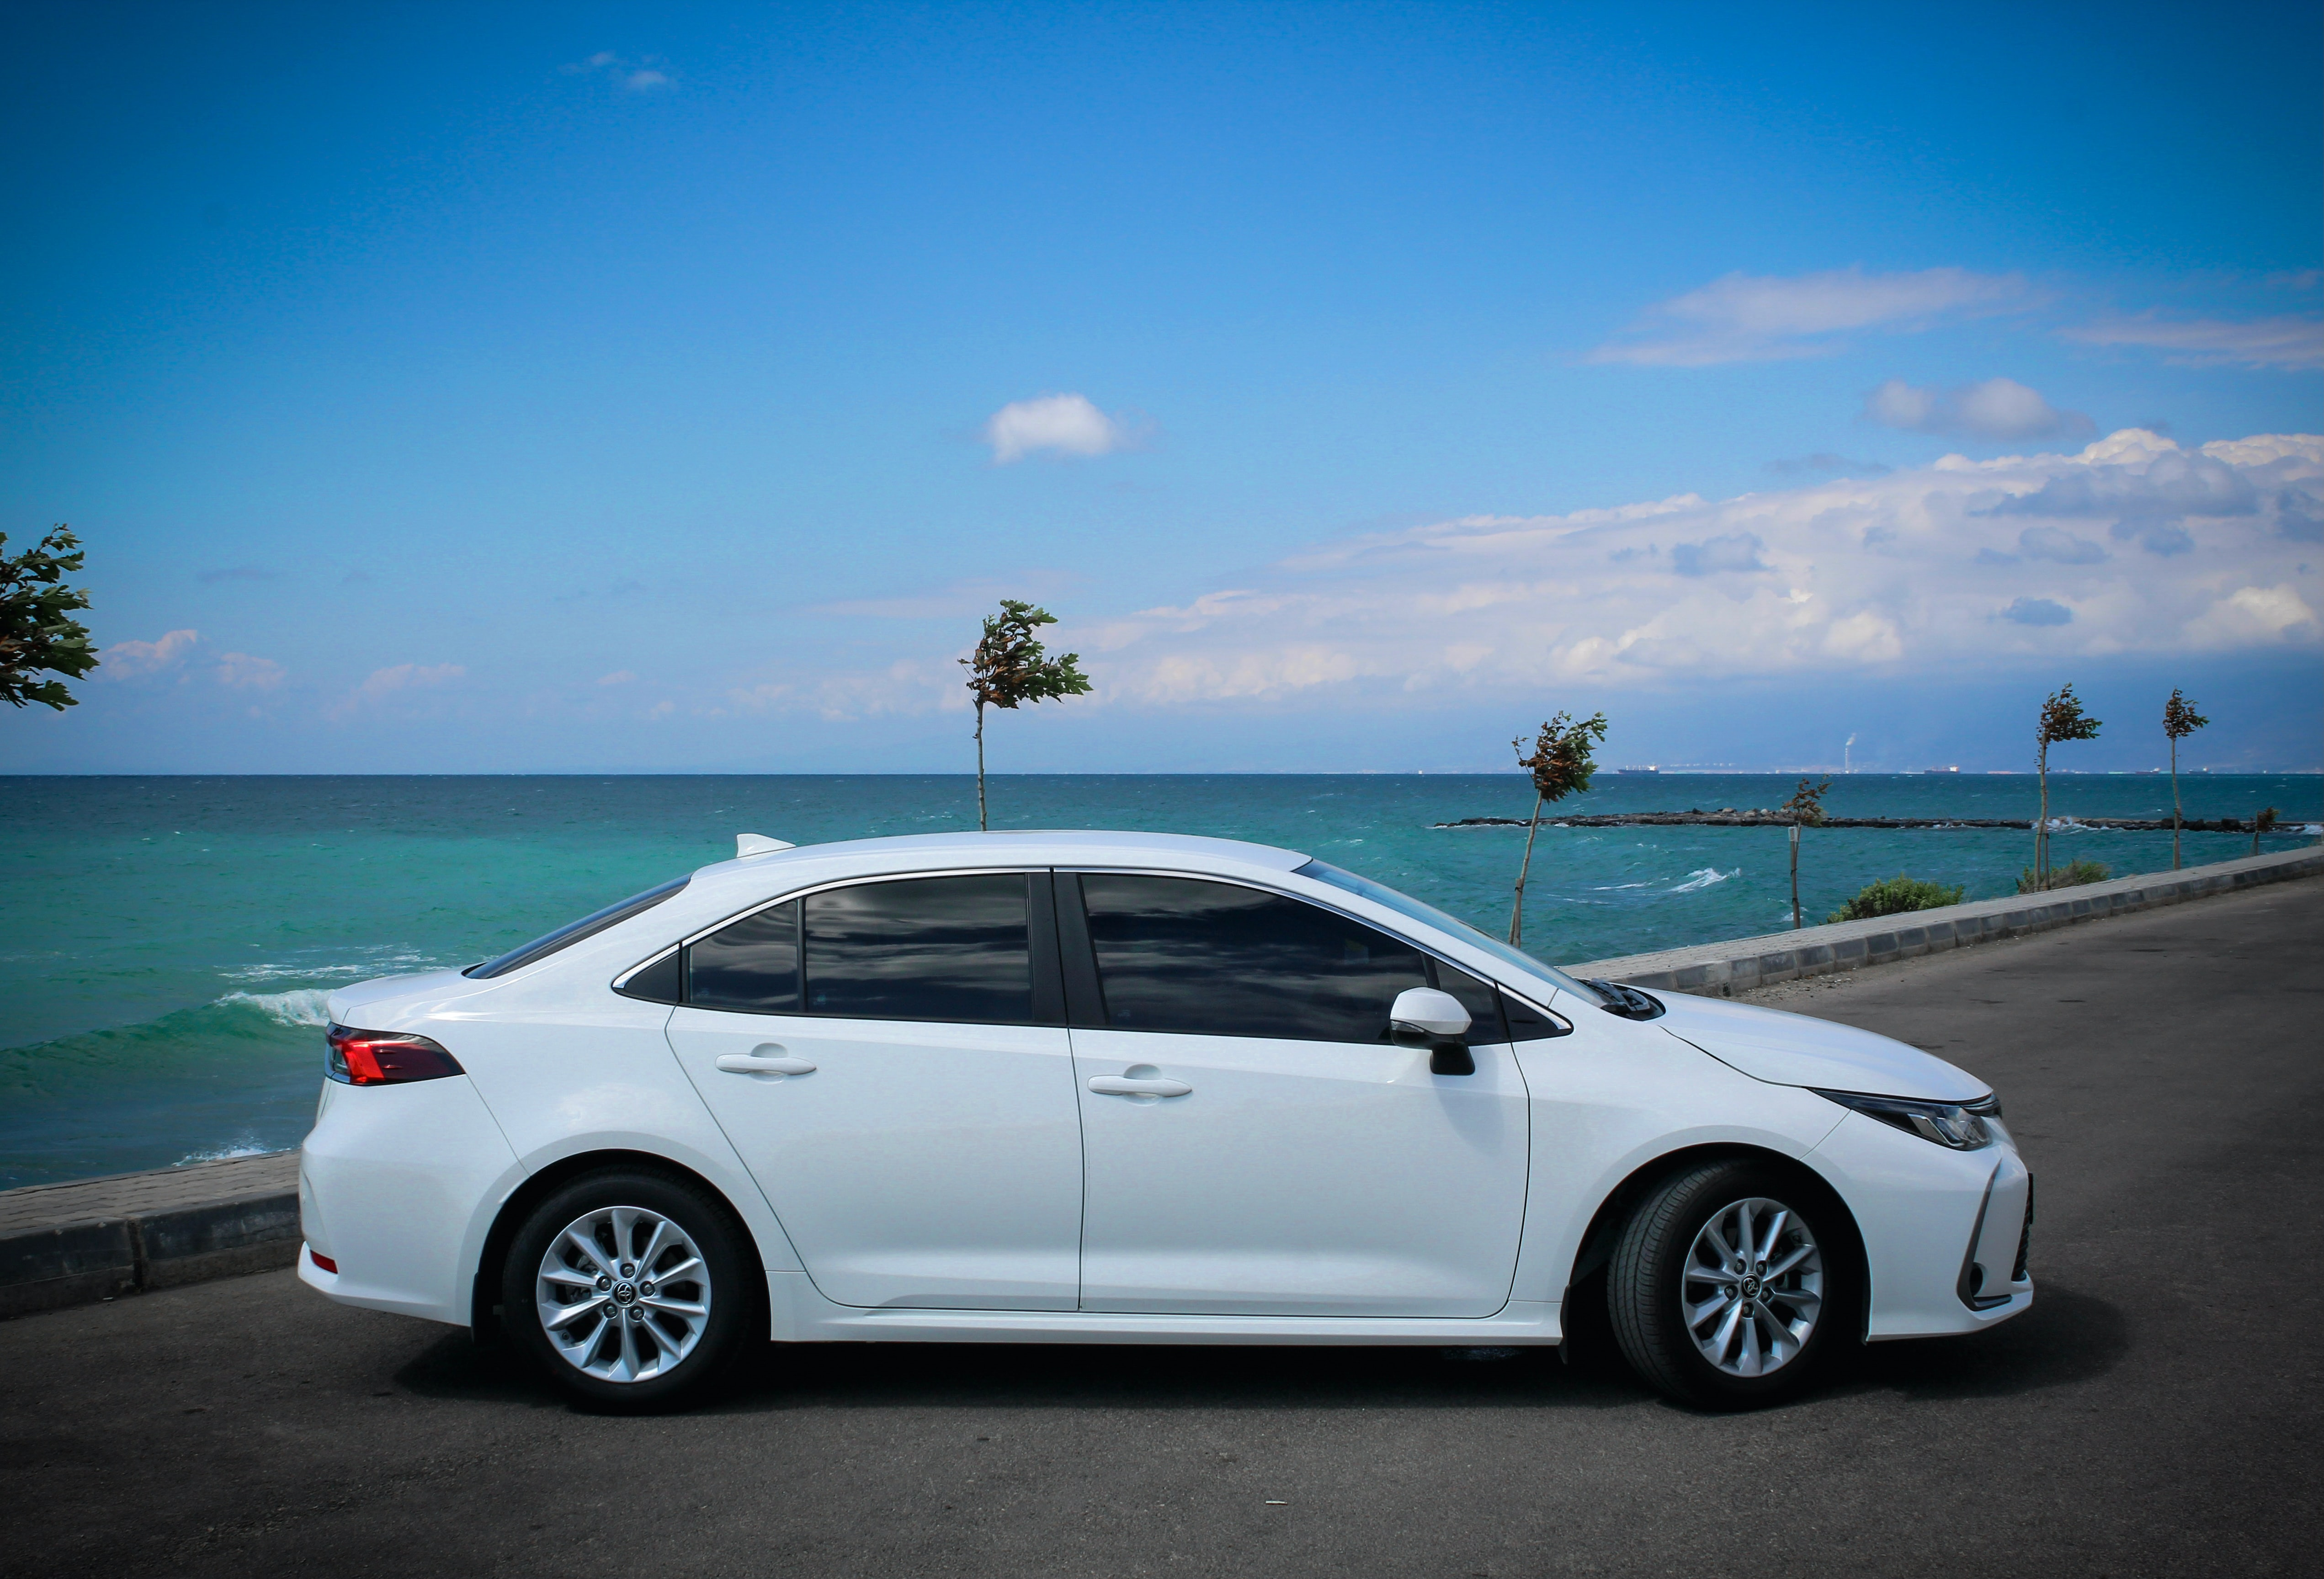
\includegraphics[width=0.7\columnwidth]{Image10}
\newline
\newline
\newline
\newline
\newline

\begin{tabular}{| m{3cm} | m{3cm} |}
\hline



Title  &  Value   \\

\hline
Camera Make  & \VAR{make10}   \\
\hline
Camera Model  & \VAR{model10}   \\
\hline
Exposure time  & \VAR{exposure_time10}  \\
\hline
aperture & \VAR{aperture10} \\
\hline

\end{tabular}


\end{center}


\end{document}